%definira klasu dokumenta 
\documentclass[12pt]{report} 

%prostor izmedu naredbi \documentclass i \begin{document} se zove uvod. U njemu se nalaze naredbe koje se odnose na cijeli dokument

%osnovni LaTex ne može riješiti sve probleme, pa se koriste različiti paketi koji olakšavaju izradu željenog dokumenta
\usepackage[croatian]{babel} 
\usepackage{amssymb}
\usepackage{amsmath}
\usepackage{txfonts}
\usepackage{mathdots}
\usepackage{titlesec}
\usepackage{array}
\usepackage{lastpage}
\usepackage{etoolbox}
\usepackage{tabularray}
\usepackage{color, colortbl}
\usepackage{adjustbox}
\usepackage{geometry}
\usepackage[classicReIm]{kpfonts}
\usepackage{hyperref}
\usepackage{fancyhdr}

\usepackage{float}
\usepackage{setspace}
\restylefloat{table}


\patchcmd{\chapter}{\thispagestyle{plain}}{\thispagestyle{fancy}}{}{} %redefiniranje stila stranice u paketu fancyhdr

%oblik naslova poglavlja
\titleformat{\chapter}{\normalfont\huge\bfseries}{\thechapter.}{20pt}{\Huge}
\titlespacing{\chapter}{0pt}{0pt}{40pt}


\linespread{1.3} %razmak između redaka

\geometry{a4paper, left=1in, top=1in,}  %oblik stranice

\hypersetup{ colorlinks, citecolor=black, filecolor=black, linkcolor=black,	urlcolor=black }   %izgled poveznice


%prored smanjen između redaka u nabrajanjima i popisima
\newenvironment{packed_enum}{
	\begin{enumerate}
		\setlength{\itemsep}{0pt}
		\setlength{\parskip}{0pt}
		\setlength{\parsep}{0pt}
	}{\end{enumerate}}

\newenvironment{packed_item}{
	\begin{itemize}
		\setlength{\itemsep}{0pt}
		\setlength{\parskip}{0pt}
		\setlength{\parsep}{0pt}
	}{\end{itemize}}




%boja za privatni i udaljeni kljuc u tablicama
\definecolor{LightBlue}{rgb}{0.9,0.9,1}
\definecolor{LightGreen}{rgb}{0.9,1,0.9}

%Promjena teksta za dugačke tablice
\DefTblrTemplate{contfoot-text}{normal}{Nastavljeno na idućoj stranici}
\SetTblrTemplate{contfoot-text}{normal}
\DefTblrTemplate{conthead-text}{normal}{(Nastavljeno)}
\SetTblrTemplate{conthead-text}{normal}
\DefTblrTemplate{middlehead,lasthead}{normal}{Nastavljeno od prethodne stranice}
\SetTblrTemplate{middlehead,lasthead}{normal}

%podesavanje zaglavlja i podnožja

\pagestyle{fancy}
\lhead{Programsko inženjerstvo}
\rhead{Digitalni poster}
\lfoot{Posterized}
\cfoot{stranica \thepage/\pageref{LastPage}}
\rfoot{\today}
\renewcommand{\headrulewidth}{0.2pt}
\renewcommand{\footrulewidth}{0.2pt}


\begin{document} 
	
	
	
	\begin{titlepage}
		\begin{center}
			\vspace*{\stretch{1.0}} %u kombinaciji s ostalim \vspace naredbama definira razmak između redaka teksta
			\LARGE Programsko inženjerstvo\\
			\large Ak. god. 2023./2024.\\
			
			\vspace*{\stretch{3.0}}
			
			\huge Digitalni poster\\
			\Large Dokumentacija, Rev. \textit{2.0}\\
			
			\vspace*{\stretch{12.0}}
			\normalsize
			Grupa: \textit{Posterized}\\
			Voditelj: \textit{Dominik Barukčić}\\
			
			
			\vspace*{\stretch{1.0}}
			Datum predaje: \textit{19. siječnja 2024.}\\
	
			\vspace*{\stretch{4.0}}
			
			Nastavnik: \textit{Miljenko Krhen}\\
		
		\end{center}

	
	\end{titlepage}

	
	\tableofcontents


	\chapter{Dnevnik promjena dokumentacije}
		
		\textbf{\textit{Kontinuirano osvježavanje}}\\
				
		
		\begin{longtblr}[
				label=none
			]{
				width = \textwidth, 
				colspec={|X[2]|X[13]|X[3]|X[3]|}, 
				rowhead = 1
			}
			\hline
			\textbf{Rev.}	& \textbf{Opis promjene/dodatka} & \textbf{Autori} & \textbf{Datum}\\[3pt] \hline
			0.1 & Napravljen predložak i dodani opisi obrazaca uporabe.	& Barukčić & 31.10.2023. 		\\[3pt] \hline 
			0.2	& Dopisane upute za povijest dokumentacije.\newline Dodane reference. & * & 24.08.2013. 	\\[3pt] \hline 
			0.5 & Dodan \textit{Use Case} dijagram i jedan sekvencijski dijagram, funkcionalni i nefunkcionalni zahtjevi i dodatak A & * & 25.08.2013. \\[3pt] \hline 
			0.6 & Arhitektura i dizajn sustava, algoritmi i strukture podataka & * & 26.08.2013. \\[3pt] \hline 
			0.8 & Povijest rada i trenutni status implementacije,\newline Zaključci i plan daljnjeg rada & * & 28.08.2013. \\[3pt] \hline 
			0.9 & Opisi obrazaca uporabe & * & 07.09.2013. \\[3pt] \hline 
			0.10 & Preveden uvod & * & 08.09.2013. \\[3pt] \hline 
			0.11 & Sekvencijski dijagrami & * & 09.09.2013. \\[3pt] \hline 
			0.12.1 & Započeo dijagrame razreda & * & 10.09.2013. \\[3pt] \hline 
			0.12.2 & Nastavak dijagrama razreda & * & 11.09.2013. \\[3pt] \hline 
			\textbf{1.0} & Verzija samo s bitnim dijelovima za 1. ciklus & * & 11.09.2013. \\[3pt] \hline 
			1.1 & Uređivanje teksta -- funkcionalni i nefunkcionalni zahtjevi & * \newline * & 14.09.2013. \\[3pt] \hline 
			1.2 & Manje izmjene:Timer - Brojilo vremena & * & 15.09.2013. \\[3pt] \hline 
			1.3 & Popravljeni dijagrami obrazaca uporabe & * & 15.09.2013. \\[3pt] \hline 
			1.5 & Generalna revizija strukture dokumenta & * & 19.09.2013. \\[3pt] \hline 
			1.5.1 & Manja revizija (dijagram razmještaja) & * & 20.09.2013. \\[3pt] \hline 
			\textbf{2.0} & Konačni tekst predloška dokumentacije  & * & 28.09.2013. \\[3pt] \hline 
			&  &  & \\[3pt] \hline	
		\end{longtblr}
	
	
		\textit{Moraju postojati glavne revizije dokumenata 1.0 i 2.0 na kraju prvog i drugog ciklusa. Između tih revizija mogu postojati manje revizije već prema tome kako se dokument bude nadopunjavao. Očekuje se da nakon svake značajnije promjene (dodatka, izmjene, uklanjanja dijelova teksta i popratnih grafičkih sadržaja) dokumenta se to zabilježi kao revizija. Npr., revizije unutar prvog ciklusa će imati oznake 0.1, 0.2, …, 0.9, 0.10, 0.11.. sve do konačne revizije prvog ciklusa 1.0. U drugom ciklusu se nastavlja s revizijama 1.1, 1.2, itd.}
	\chapter{Opis projektnog zadatka}
		
		Razvijamo aplikaciju namijenjenu sudionicima stručne konferencije, s ciljem pojednostavljenja pregleda i ocjenjivanja radova. Naša misija je stvoriti integrirano digitalno okruženje koje potiče interakciju između sudionika i autora te promiče znanstveni i stručni dijalog. U skladu s tim, implementiramo ključne korisničke zahtjeve kako bismo osigurali optimalno korisničko iskustvo i funkcionalnost sustava.
		
		Potrebno je izgraditi sustav za naručitelje kojim bi se održane konferencije mogle pratiti putem aplikacije. Aplikacija je sustav preko kojeg se mogu pregledavati sadržaji poput postera i radova autora. Svaki autor može prijaviti svoj rad i administratoru konferencije proslijediti materijale potrebne za stavljanje svog rada u aplikaciju. Za svaki pojedini rad, korisnik ima priliku glasati u cilju biranja 3 najbolja rada. Tijekom održavanja konferencije, na aplikaciji postoji video prijenos u stvarnom vremenu te konferencije. Na kraju i tijekom održavanja konferencije svaki korisnik može preuzeti fotografije s konferencije.
		
		Ključni zahtjev je omogućiti istovremeni rad više korisnika u stvarnom vremenu bez gubitka performansi. Na primjer, dok jedan sudionik pregledava rad, drugi može istovremeno davati svoje ocjene ili komentare. Ova funkcionalnost je ključna za dinamičnu interakciju i suradnju među sudionicima konferencije.
		
		Još jedan važan zahtjev je brz pristup bazi podataka. Kada korisnici pristupe aplikaciji za pretraživanje radova ili unos svojih glasova, odziv sustava mora biti brz i učinkovit. Ovaj zahtjev osigurava korisnicima bolje korisničko iskustvo smanjenjem vremena čekanja na učitavanje informacija, što je posebno važno u okruženju konferencije gdje je vrijeme sudionika dragocjeno.
		
		Naša aplikacija ima sigurnu, brzu i pouzdanu komunikaciju s bazom podataka i stabilnost veze sa serverom. Pružamo zaštitu povjerljivih podataka konferencije i korisnika te osiguravanje neprekidnog rada aplikacije.
		
		\newpage
		
		Sustav je prilagođen za rad na mobilnim uređajima. Aplikacija je prilagodljiva i lako koristiva na različitim veličinama ekrana, od pametnih telefona do tableta. Sudionicima se omogućava da pristupe i koriste aplikaciju bilo kada i bilo gdje, što je posebno važno u današnjem mobilnom i povezanom svijetu.
		
		Svi ovi zahtjevi su usmjereni na stvaranje korisničkog iskustva koje je učinkovito, intuitivno i prilagođeno potrebama sudionika stručne konferencije. Cilj nam je osigurati da aplikacija ispuni očekivanja korisnika pružajući inovativnu platformu za razmjenu znanstvenih i stručnih informacija.
		
		Brojne su koristi ovog projekta, a one kojima naš sustav pridonosi su: 
		
		\begin{packed_item}
			\item Povećana interaktivnost: omogućuje aktivnije sudjelovanje posjetitelja kroz glasovanje i povratne informacije.
			\item Bolja organizacija: automatizira prijavu radova i administrativne procese, štedeći vrijeme i resurse.
			\item Pristupačnost: digitalizacija sadržaja konferencije osigurava lakši pristup informacijama za sve sudionike.
			\item Ekološka održivost: smanjenje upotrebe papira kroz digitalne postere i materijale.
			\item Analitički podaci: skupljanje podataka o preferencijama sudionika, korisnih za buduće događaje.
		\end{packed_item}

		Postoje razna slična rješenja ovakvih platformu poput Whova, EventMobi, i Attendify. Međutim, naša aplikacija se razlikuje specifičnim funkcijama poput prilagođenog glasovanja, notifikacija i integracije s lokalnim vremenskim uvjetima, što je prilagođeno specifičnim potrebama naše ciljane konferencije.
		
		Korisnici ove aplikacije i zahtjevi svakog korisnika:
		\begin{packed_item}
			\item Posjetitelji konferencije: željni pristupa sadržaju i interakcije.
			\item Autori radova: traže platformu za predstavljanje rada i dobivanje povratnih informacija.
			\item Organizatori konferencija: teže efikasnom upravljanju sadržajem i interakcijom sudionika.
			\item Sponzori: žele promovirati svoje brendove putem aplikacije.
		\end{packed_item}
		Aplikacija će biti dizajnirana modularno, omogućujući prilagodbu za različite tipove konferencija, broj sudionika, i specifične zahtjeve organizatora. Projekt uključuje razvoj i implementaciju aplikacije, testiranje funkcionalnosti, te suradnju s krajnjim korisnicima za povratne informacije i unaprjeđenja.
		
		\newpage
		
		Postoje razne nadogradnje našeg projektnog zadatka, a neka od njih su sinteza sustava s ovim tehnologijama:
		\begin{packed_item}
			\item Umjetna inteligencija: personalizirani prijedlozi sesija bazirani na interesima korisnika.
			\item Virtualna stvarnost: mogućnost virtualnog obilaska konferencije za korisnike koji ne mogu prisustvovati fizički.
			\item Integracija s društvenim mrežama: olakšavanje dijeljenja sadržaja i povećanje vidljivosti konferencije.
		\end{packed_item}

		
		
		\eject
		
		
	
	\chapter{Specifikacija programske potpore}
		
	\section{Funkcionalni zahtjevi}
			
%			\textbf{\textit{dio 1. revizije}}\\
			
%			\textit{Navesti \textbf{dionike} koji imaju \textbf{interes u ovom sustavu} ili  \textbf{su nositelji odgovornosti}. To su prije svega korisnici, ali i administratori sustava, naručitelji, razvojni tim.}\\
				
%			\textit{Navesti \textbf{aktore} koji izravno \textbf{koriste} ili \textbf{komuniciraju sa sustavom}. Oni mogu imati inicijatorsku ulogu, tj. započinju određene procese u sustavu ili samo sudioničku ulogu, tj. obavljaju određeni posao. Za svakog aktora navesti funkcionalne zahtjeve koji se na njega odnose.}\\
			
			
			\noindent \textbf{Dionici:}
			
			\begin{packed_enum}
				
				\item Naručitelj
				\item Administrator
				\item Neregistrirani korisnik	
				\item Registrirani korisnik
				\item Razvojni tim
				
			\end{packed_enum}
			
			\noindent \textbf{Aktori i njihovi funkcionalni zahtjevi:}
			
			
			\begin{packed_enum}
				\item  \underbar{Administrator (inicijator) može:}
				
				\begin{packed_enum}
					
					\item dodati autore, radove, pokrovitelje konferencije i lokacije
					\item uređivati podatke konferencije
					\item započeti i završiti konferenciju
					\item postaviti fotografije koje su slikane tijekom konferencije u galeriju
					\item objaviti rezultate konferencije
					
				\end{packed_enum}
			
				\item  \underbar{Neregistrirani korisnik (inicijator) može:}
				
				\begin{packed_enum}
					
					\item pristupiti sustavu
					\item unijeti lozinku za pristup konferenciji
					\item registrirati se u sustav
					
				\end{packed_enum}
				
				\item  \underbar{Registrirani korisnik (inicijator) može:}
				
				\begin{packed_enum}
					
					\item prijaviti se u sustav
					\item pregledavati promotivne materijale pokrovitelja konferencije
					\item pregledavati radove sudionika
					\item glasati za jedan rad
					\item uz pomoć direktnog video prijenosa pratiti trenutna događanja u glavnoj konferencijskoj dvorani
					\item pregledavati i spremati fotografije iz galeriji
					\item vidjeti mjesto održavanje konferencije i podatke o trenutnim vremenskim uvjetima
					\item vidjeti konačne reultate konferencije
					
				\end{packed_enum}
					
				\item  \underbar{Baza podataka (sudionik) obavlja:}
					
				\begin{packed_enum}
						
					\item pohranjuje sve podatke o korisnicima
					\item pohranjuje sve podatke o autorima i njihovim radovima
					\item pohranjuje sve podatke o konferencijama
					\item pohranjuje sve podatke o mjestu održavanja
					\item pohranjuje sve podatke o fotografijama slikanim tijekom konferencije i pokroviteljima
						
				\end{packed_enum}
				
			\end{packed_enum}
			
			\eject 
			
			
				
			\subsection{Obrasci uporabe}
				
%				\textbf{\textit{dio 1. revizije}}
				
%				\subsubsection{Opis obrazaca uporabe}
				
%					\noindent \underbar{\textbf{UC$<$broj obrasca$>$ -$<$ime obrasca$>$}}
%					\begin{packed_item}
	
%						\item \textbf{Glavni sudionik: }$<$sudionik$>$
%						\item  \textbf{Cilj:} $<$cilj$>$
%						\item  \textbf{Sudionici:} $<$sudionici$>$
%						\item  \textbf{Preduvjet:} $<$preduvjet$>$
%						\item  \textbf{Opis osnovnog tijeka:}
						
%						\item[] \begin{packed_enum}
	
%							\item $<$opis korak jedan$>$
%							\item $<$opis korak dva$>$
%							\item $<$opis korak tri$>$
%							\item $<$opis korak četiri$>$
%							\item $<$opis korak pet$>$
%						\end{packed_enum}
						
%						\item  \textbf{Opis mogućih odstupanja:}
						
%						\item[] \begin{packed_item}
	
%							\item[2.a] $<$opis mogućeg scenarija odstupanja u koraku 2$>$
%							\item[] \begin{packed_enum}
								
%								\item $<$opis rješenja mogućeg scenarija korak 1$>$
%								\item $<$opis rješenja mogućeg scenarija korak 2$>$
								
%							\end{packed_enum}
%							\item[2.b] $<$opis mogućeg scenarija odstupanja u koraku 2$>$
%							\item[3.a] $<$opis mogućeg scenarija odstupanja  u koraku 3$>$
							
%						\end{packed_item}
%					\end{packed_item}

					\noindent \underbar{\textbf{UC1 - Stvaranje konferencije i dodjela administratora}}
					\begin{packed_item}
	
						\item \textbf{Glavni sudionik: }Super Administrator
						\item  \textbf{Cilj:} Stvoriti konferenciju i dodijeliti je administratoru.
						\item  \textbf{Sudionici:} Baza podataka
						\item  \textbf{Preduvjet:} -
						\item  \textbf{Opis osnovnog tijeka:}
						
						\item[] \begin{packed_enum}
	
							\item Super Administrator stvara konferenciju.
							\item Pridjeljuje ovlasti nad konferencijom odabranom administratoru.
						\end{packed_enum}
						
						\item  \textbf{Opis mogućih odstupanja:}
						
						\item[] \begin{packed_item}
	
							\item[2.a] Administrator ne postoji
							\item[] \begin{packed_enum}
								
								\item Super Administrator stvara Administratora i ponavlja postupak.
								
							\end{packed_enum}
							
						\end{packed_item}
					\end{packed_item}

					\noindent \underbar{\textbf{UC2 - Unos podataka o konferenciji}}
					\begin{packed_item}
						
						\item \textbf{Glavni sudionik: }Administrator
						\item  \textbf{Cilj:} Dodati podatke o konferenciji u bazu podataka.
						\item  \textbf{Sudionici:} Baza podataka
						\item  \textbf{Preduvjet:} -
						\item  \textbf{Opis osnovnog tijeka:}
						
						\item[] \begin{packed_enum}
							
							\item Administrator unosi podatke o konferenciji i mjestu održavanja.
							\item Podaci se pohranjuju u bazu podataka.
					
						\end{packed_enum}
							
					\end{packed_item}

					\noindent \underbar{\textbf{UC3 - Unos podataka o autoru i radu}}
					\begin{packed_item}
						
						\item \textbf{Glavni sudionik: }Administrator
						\item  \textbf{Cilj:} Dodati podatke o autoru i radu u bazu podataka.
						\item  \textbf{Sudionici:} Baza podataka
						\item  \textbf{Preduvjet:} -
						\item  \textbf{Opis osnovnog tijeka:}
						
						\item[] \begin{packed_enum}
							
							\item Administrator unosi podatke o autoru i radu preko grafičkog sučelja.
							\item Aplikacija dodaje podatke u bazu podataka.
					
						\end{packed_enum}
		
					\end{packed_item}

					\noindent \underbar{\textbf{UC4 - Početak konferencije}}
					\begin{packed_item}
						
						\item \textbf{Glavni sudionik: }Administrator
						\item  \textbf{Cilj:} Omogućiti korisnicima pristup konferenciji, pregled radova i glasovanje.
						\item  \textbf{Sudionici:} Baza podataka
						\item  \textbf{Preduvjet:} Uneseni su svi potrebni podaci o konferenciji.
						\item  \textbf{Opis osnovnog tijeka:}
						
						\item[] \begin{packed_enum}
							
							\item Administrator započinje konferenciju.

						\end{packed_enum}
							
					\end{packed_item}

					\noindent \underbar{\textbf{UC5 - Dodavanje fotografija u galeriju}}
					\begin{packed_item}
						
						\item \textbf{Glavni sudionik: }Administrator
						\item  \textbf{Cilj:} Dodati fotografije konferencije u galeriju.
						\item  \textbf{Sudionici:} Baza podataka
						\item  \textbf{Preduvjet:} Konferencija postoji.
						\item  \textbf{Opis osnovnog tijeka:}
						
						\item[] \begin{packed_enum}
							
							\item Administrator tijekom i nakon konferencije dodaje fotografije pomoću grafičkog sučelja.
							\item Aplikacija pohranjuje osnovne podatke o fotografijama u bazu podataka.

						\end{packed_enum}
							
					\end{packed_item}
					
					\noindent \underbar{\textbf{UC6 - Registracija}}
					\begin{packed_item}
						
						\item \textbf{Glavni sudionik: }Neregistrirani korisnik
						\item  \textbf{Cilj:} Registrirati se u sustavu kako bi se omogućio pristup svim funkcionalnostima aplikacije.
						\item  \textbf{Sudionici:} Baza podataka
						\item  \textbf{Preduvjet:} Korisnik ima dobiven pin.
						\item  \textbf{Opis osnovnog tijeka:}
						
						\item[] \begin{packed_enum}
							
							\item Korisnik pristupa registracijskoj stranici aplikacije.
							\item Unosi svoje osobne podatke za registraciju.
							\item Sustav provjerava podatke i stvara račun.
							\item Korisnik prima potvrdu o uspješnoj registraciji i pristupa stranici konferencije.
						\end{packed_enum}
						
						\item  \textbf{Opis mogućih odstupanja:}
						
						\item[] \begin{packed_item}
							
							\item[3.a] Uneseni podaci nepotpuni ili neispravni.
							\item[] \begin{packed_enum}
								
								\item Sustav prikazuje upozorenje i traži ispravak podataka.
								
							\end{packed_enum}
						\end{packed_item}
					\end{packed_item}
					
					\noindent \underbar{\textbf{UC7 - Prijava u sustav}}
					\begin{packed_item}
						
						\item \textbf{Glavni sudionik: }Registrirani korisnik
						\item  \textbf{Cilj:} Prijaviti se u sustav kako bi se pristupilo konferenciji.
						\item  \textbf{Sudionici:} Baza podataka
						\item  \textbf{Preduvjet:} Korisnik ima korisnički račun.
						\item  \textbf{Opis osnovnog tijeka:}
						
						\item[] \begin{packed_enum}
							
							\item Korisnik pristupa stranici za prijavu u aplikaciju.
							\item Unosi svoje korisničko ime i lozinku.
							\item Sustav provjerava unesene podatke i omogućuje pristup konferenciji.
						\end{packed_enum}
						
						\item  \textbf{Opis mogućih odstupanja:}
						
						\item[] \begin{packed_item}
							
							\item[3.a] Uneseni podaci su netočni.
							\item[] \begin{packed_enum}
								
								\item Sustav prikazuje upozorenje o neuspjeloj prijavi i traži ponovni upis podataka.
								
							\end{packed_enum}

						\end{packed_item}
					\end{packed_item}
					
					\noindent \underbar{\textbf{UC8 - Pregled radova sudionika}}
					\begin{packed_item}
						
						\item \textbf{Glavni sudionik: }Registrirani korisnik
						\item  \textbf{Cilj:} Pregledati radove sudionika konferencije.
						\item  \textbf{Sudionici:} Baza podataka
						\item  \textbf{Preduvjet:} Korisnik je prijavljen u sustav.
						\item  \textbf{Opis osnovnog tijeka:}
						
						\item[] \begin{packed_enum}
							
							\item Korisnik pristupa dijelu aplikacije koji prikazuje sve dostupne radove sudionika.
							\item Korisnik pregledava pojedinačne radove.

						\end{packed_enum}
							
					\end{packed_item}

					\noindent \underbar{\textbf{UC9 -  Glasovanje za rad}}
					\begin{packed_item}
						
						\item \textbf{Glavni sudionik: }Registrirani korisnik
						\item  \textbf{Cilj:} Dati svoj glas određenom posteru na konferenciji.
						\item  \textbf{Sudionici:} Baza podataka
						\item  \textbf{Preduvjet:} Korisnik je prijavljen u sustavu i konferencija je u tijeku.
						\item  \textbf{Opis osnovnog tijeka:}
						
						\item[] \begin{packed_enum}
							
							\item Korisnik odabire rad za koji će glasati.
							\item Sustav bilježi glas korisnika za odabrani poster.
							
						\end{packed_enum}
						
						\item  \textbf{Opis mogućih odstupanja:}
						
						\item[] \begin{packed_item}
							
							\item[2.a] Korisnik je već glasovao.
							\item[] \begin{packed_enum}
								
								\item Sustav ne bilježi glas i pokazuje upozorenje da je moguće samo jednom glasovati.
								
							\end{packed_enum}
							
						\end{packed_item}
					\end{packed_item}

					\noindent \underbar{\textbf{UC10 - Pregled fotografija u galeriji}}
					\begin{packed_item}
						\item \textbf{Glavni sudionik: }Registrirani korisnik
						\item \textbf{Cilj:} Pregledati fotografije snimljene tijekom konferencije.
						\item \textbf{Sudionici:} Baza podataka
						\item \textbf{Preduvjet:} Korisnik je prijavljen u sustav.
						\item \textbf{Opis osnovnog tijeka:}
						
						\begin{packed_enum}
							\item Korisnik pristupa dijelu aplikacije koji prikazuje dostupne fotografije s konferencije.
							\item Korisnik pregledava dostupne fotografije.
						\end{packed_enum}
					\end{packed_item}				
					
					\noindent \underbar{\textbf{UC11 - Spremanje fotografija na svoj uređaj}}
					\begin{packed_item}
						\item \textbf{Glavni sudionik: }Registrirani korisnik
						\item \textbf{Cilj:} Spremiti odabrane fotografije na svoj uređaj.
						\item \textbf{Sudionici:} Baza podataka
						\item \textbf{Preduvjet:} Korisnik je prijavljen u sustav i pregledava fotografije.
						\item \textbf{Opis osnovnog tijeka:}
						
						\begin{packed_enum}
							\item Korisnik pregledava fotografije.
							\item Korisnik odabire fotografiju koju želi spremiti i preuzima ju na svoj uređaj.
						\end{packed_enum}
					\end{packed_item}	
					
					\noindent \underbar{\textbf{UC12 - Direktno video praćenje konferencije}}
					\begin{packed_item}
						\item \textbf{Glavni sudionik: }Registrirani korisnik
						\item \textbf{Cilj:} Pratiti video prijenos događanja konferencije u stvarnom vremenu.
						\item \textbf{Sudionici:} Baza podataka
						\item \textbf{Preduvjet:} Korisnik je prijavljen u sustav i ima stabilnu internetsku vezu.
						\item \textbf{Opis osnovnog tijeka:}
						
						\begin{packed_enum}
							\item Registrirani korisnik pristupa opciji "Direktno video praćenje" u aplikaciji.
							\item Sustav prikazuje video prijenos za praćenje.
						\end{packed_enum}
						
						\item \textbf{Opis mogućih odstupanja:}
						
						\begin{packed_item}
							\item[2.a] Korisnik nema stabilnu internetsku vezu.
							\begin{packed_enum}
								\item Sustav obavještava korisnika da je potrebna stabilna internetska veza za praćenje video prijenosa.
							\end{packed_enum}
						\end{packed_item}
					\end{packed_item}
					
					\noindent \underbar{\textbf{UC13 - Završetak konferencije}}
					\begin{packed_item}
						
						\item \textbf{Glavni sudionik: }Administrator
						\item  \textbf{Cilj:} Završiti konferenciju i prekinuti mogućnost glasovanja.
						\item  \textbf{Sudionici:} Baza podataka
						\item  \textbf{Preduvjet:} -
						\item  \textbf{Opis osnovnog tijeka:}
						
						\item[] \begin{packed_enum}
							
							\item Administrator završava konferenciju.
							\item Zbrajaju se glasovi.

						\end{packed_enum}
						
					\end{packed_item}
					
					\noindent \underbar{\textbf{UC14 - Slanje obavijest o uspjehu i dodjeli nagrada}}
					\begin{packed_item}
						
						\item \textbf{Glavni sudionik: }Administrator
						\item  \textbf{Cilj:} Poslati e-mail autorima o njihovom uspjehu i pozivnicu na dodjelu nagrada za prva tri rada svim korisnicima i autorima.
						\item  \textbf{Sudionici:} Baza podataka
						\item  \textbf{Preduvjet:} Konferencija je završila.
						\item  \textbf{Opis osnovnog tijeka:}
						
						\item[] \begin{packed_enum}
							
							\item Administrator šalje e-mail svim autorima u kojem ih obavještava o njihovom rangu prema zabilježenim glasovima i o mjestu i vremenu dodjele nagrada za prva tri rada.
							\item Administrator obavještava sve korisnike o mjestu i vremenu dodjele nagrada.
						\end{packed_enum}
						
					\end{packed_item}
					
					
				\subsubsection{Dijagrami obrazaca uporabe}
					
%					\textit{Prikazati odnos aktora i obrazaca uporabe odgovarajućim UML dijagramom. Nije nužno nacrtati sve na jednom dijagramu. Modelirati po razinama apstrakcije i skupovima srodnih funkcionalnosti.}
					
					\begin{figure}[H]
						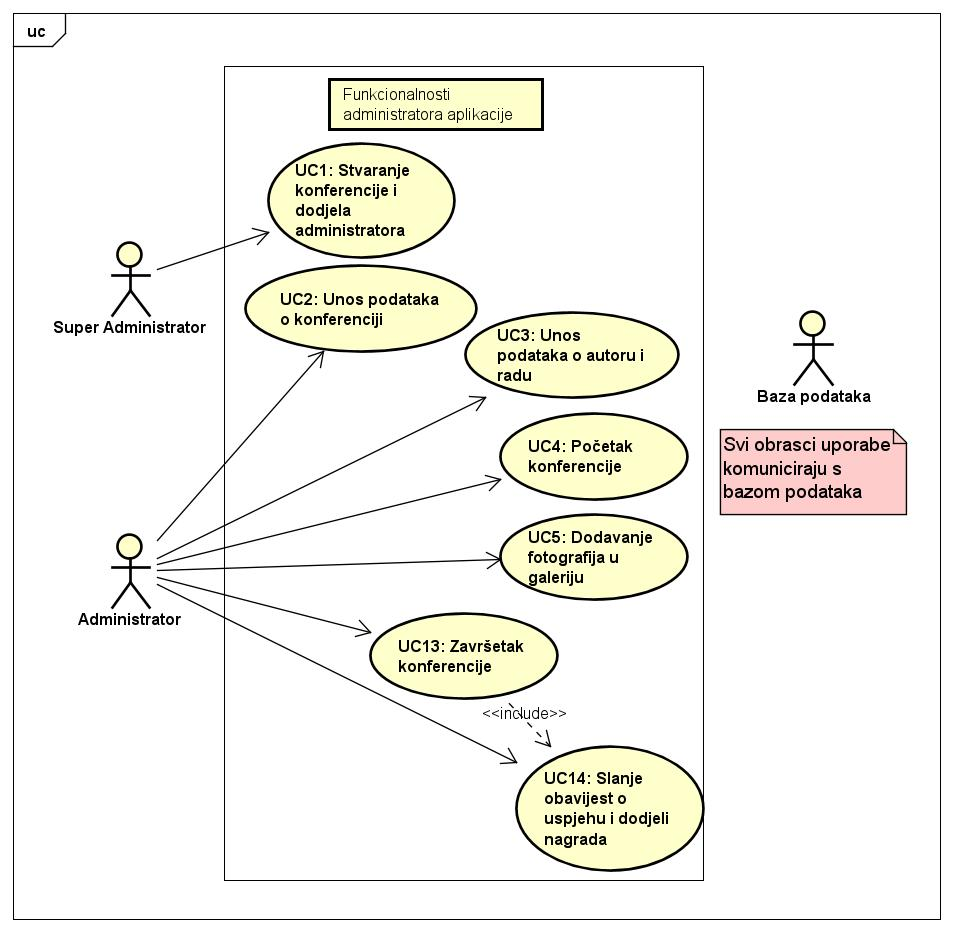
\includegraphics[scale=0.45]{dijagrami/UC_dijagram_administrator.JPG} %veličina slike u odnosu na originalnu datoteku i pozicija slike
						\centering
						\caption{Dijagram obrazaca uporabe - administrator}
						\label{fig:promjene}
					\end{figure}
					\begin{figure}[H]
						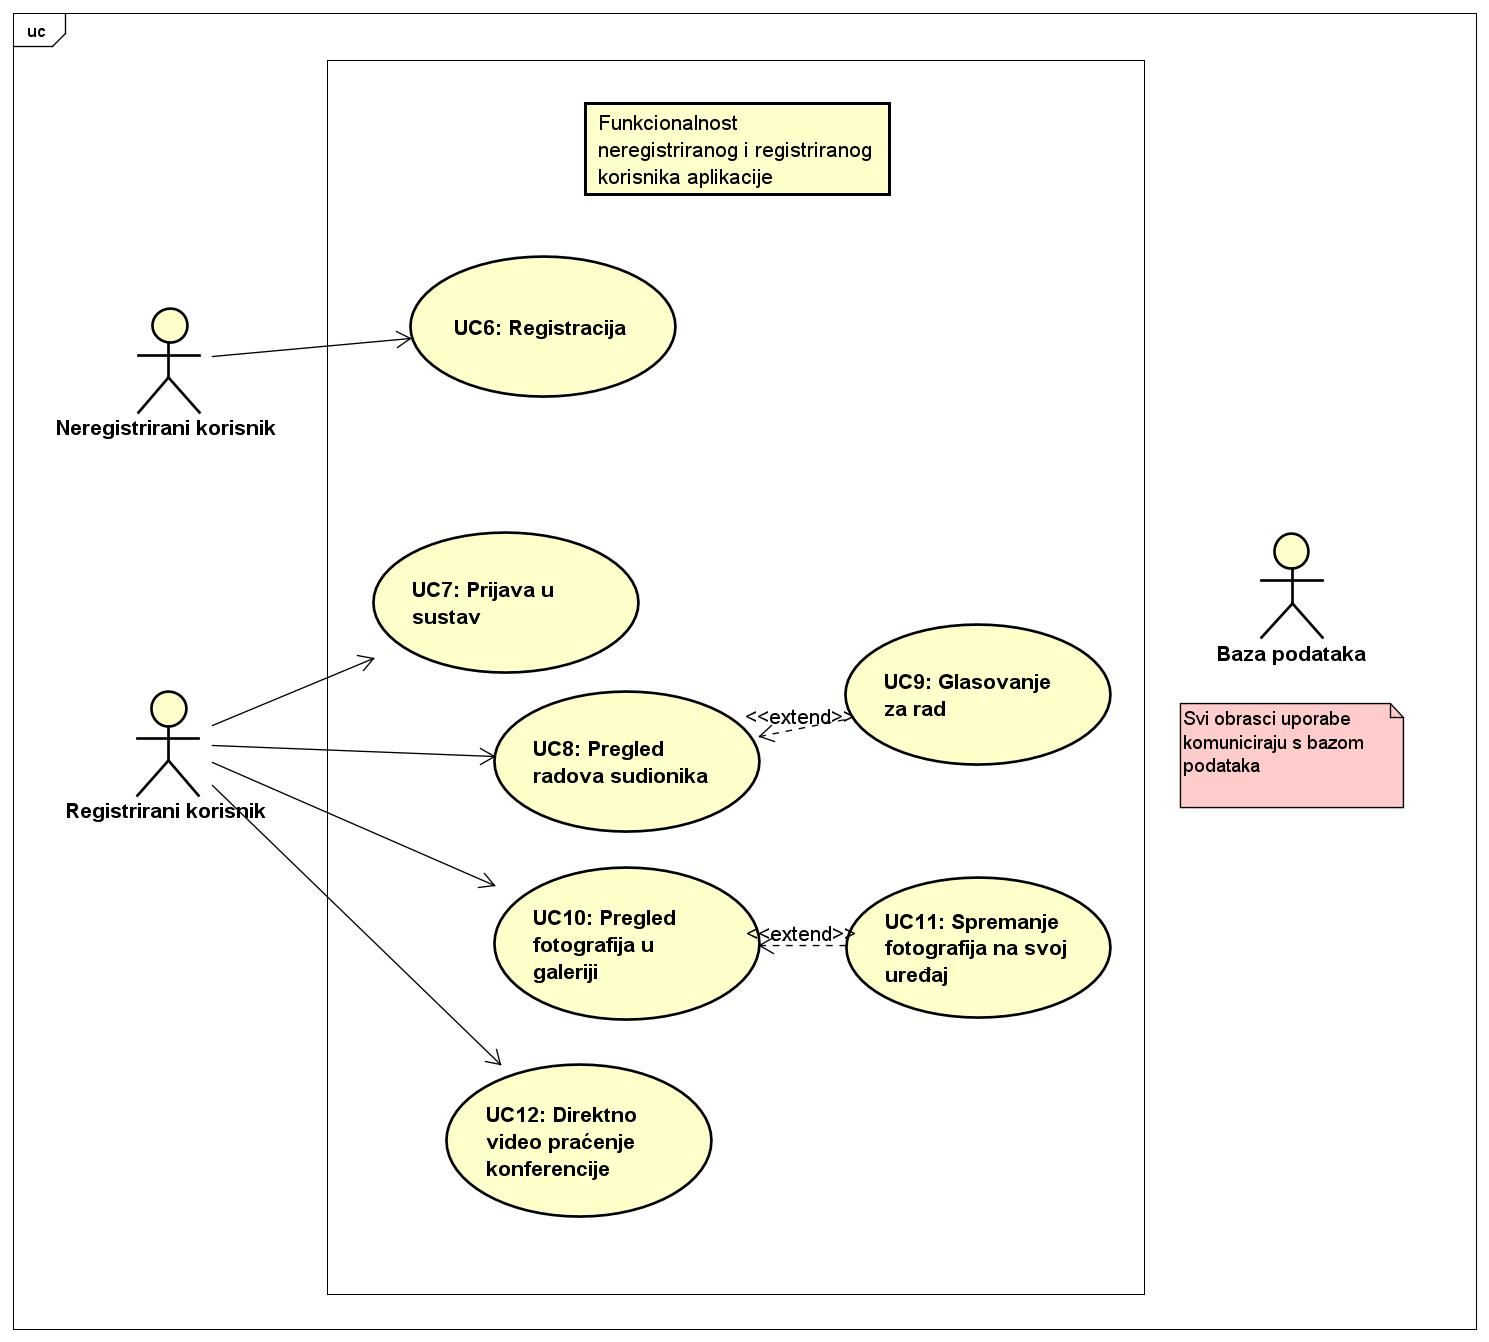
\includegraphics[scale=0.3]{dijagrami/UC_dijagram_korisnik.JPG} %veličina slike u odnosu na originalnu datoteku i pozicija slike
						\centering
						\caption{Dijagram obrazaca uporabe - korisnici}
						\label{fig:promjene2}
					\end{figure}
				\eject		
				
			\subsection{Sekvencijski dijagrami}
				\hspace{0.5cm} Korisnik pokreće aplikaciju. Ima ograničen pristup sadržajima aplikacije sve dok ne upiše pin koji je dodijeljen sudionicima konferencije. Upisani pin se zatim provjerava i korisnik nastavlja na stranicu za prijavu/registraciju.
				
				Kad korisnik ima stvoreni račun, prijavljuje se u aplikaciju pomoću adrese elektroničke pošte i lozinke. Prijavljeni korisnik onda može pristupiti sadržaju konferencije. 
				
				Za vrijeme sudjelovanja na konferenciji korisnik može pregledavati sadržaj konferencije i radove. Korisnik može glasovati samo za jedan rad i pratiti video prijenos trenutnih događanja u glavnoj konferencijskoj dvorani u realnom vremenu. Također ima dostupno pregledavanje i preuzimanje slika s konferencije - tijekom i nakon što konferencija završi. Korisnik može ugasiti aplikaciju kad god ima potrebu za tim.
				
				Dijagram je prikazan na sljedećoj stranici.
				\eject
				
				\begin{figure}[H]
					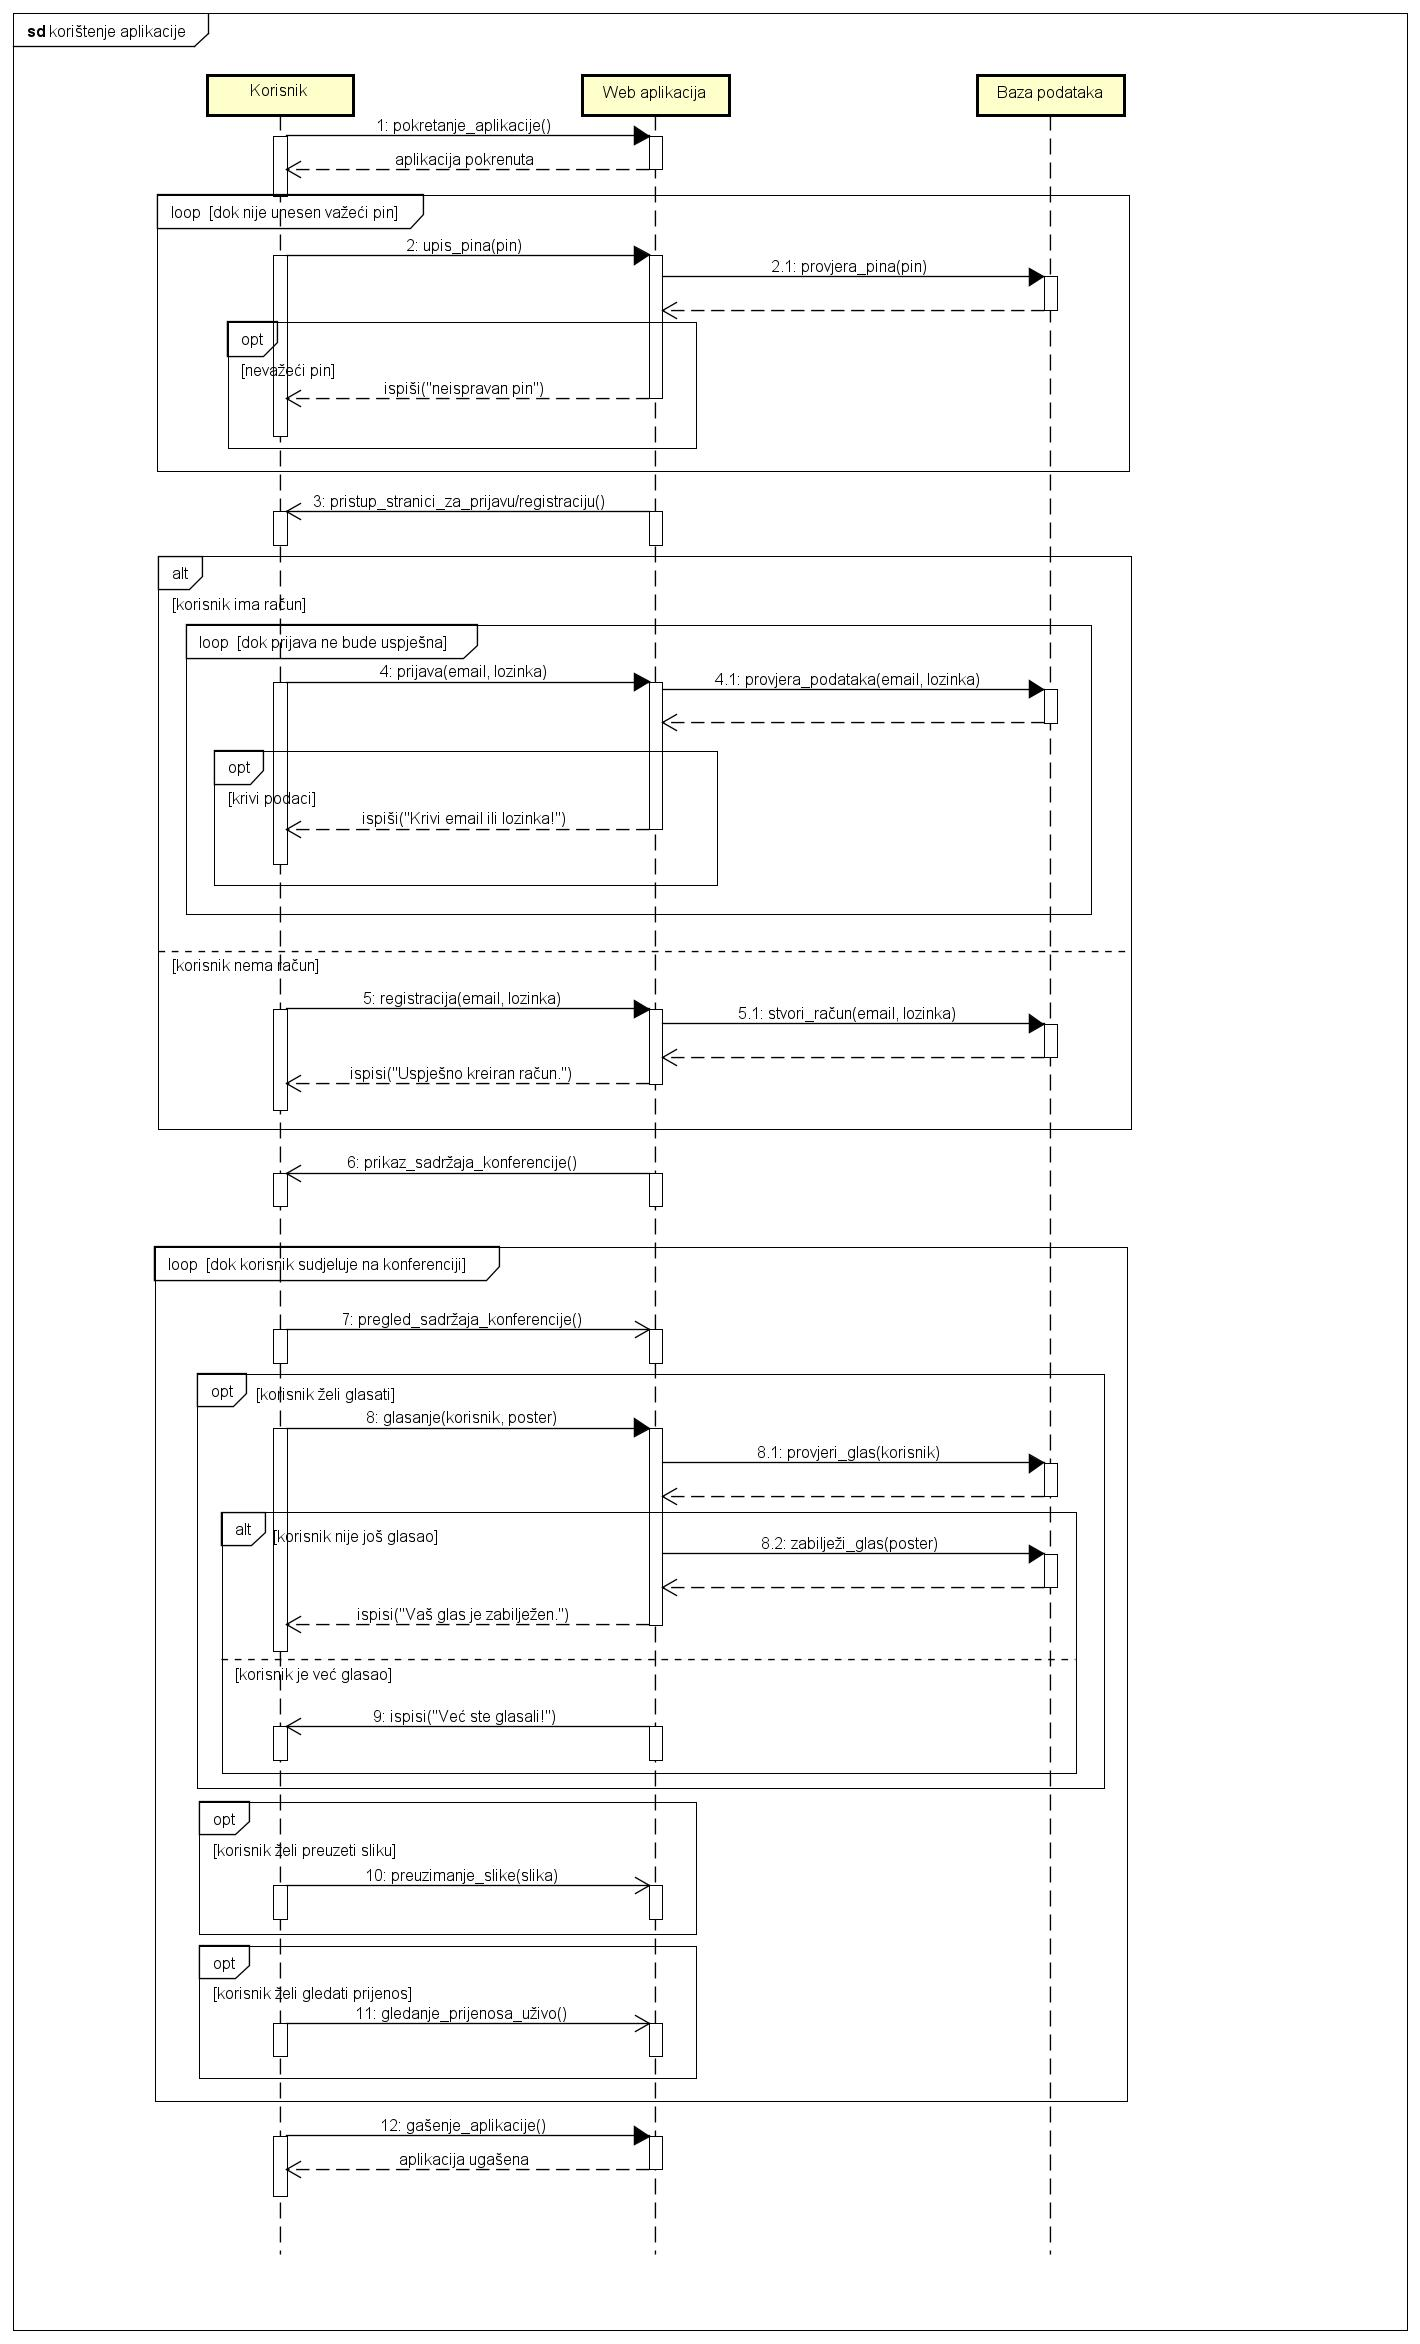
\includegraphics[scale=0.28]{dijagrami/koristenje_aplikacije.JPG} %veličina slike u odnosu na originalnu datoteku i pozicija slike
					\centering
					\caption{Sekvencijski dijagram korištenja aplikacije}
					\label{fig:promjene}
				\end{figure}

				Administrator dodaje autore i njihove radove prije početka konferencije. Nadodaje ih dok ne doda sve sudionike (autore) i njihove radove.
				Zatim dodaje sponzore konferencije dok ih sve ne upiše.

				Administrator započinje konferenciju. Tijekom konferencije administrator ima mogućnost dodavanja fotografija te konferencije. Administrator završava konferenciju. 

				Administrator dodaje fotografije i nakon konferencije.

				\begin{figure}[H]
					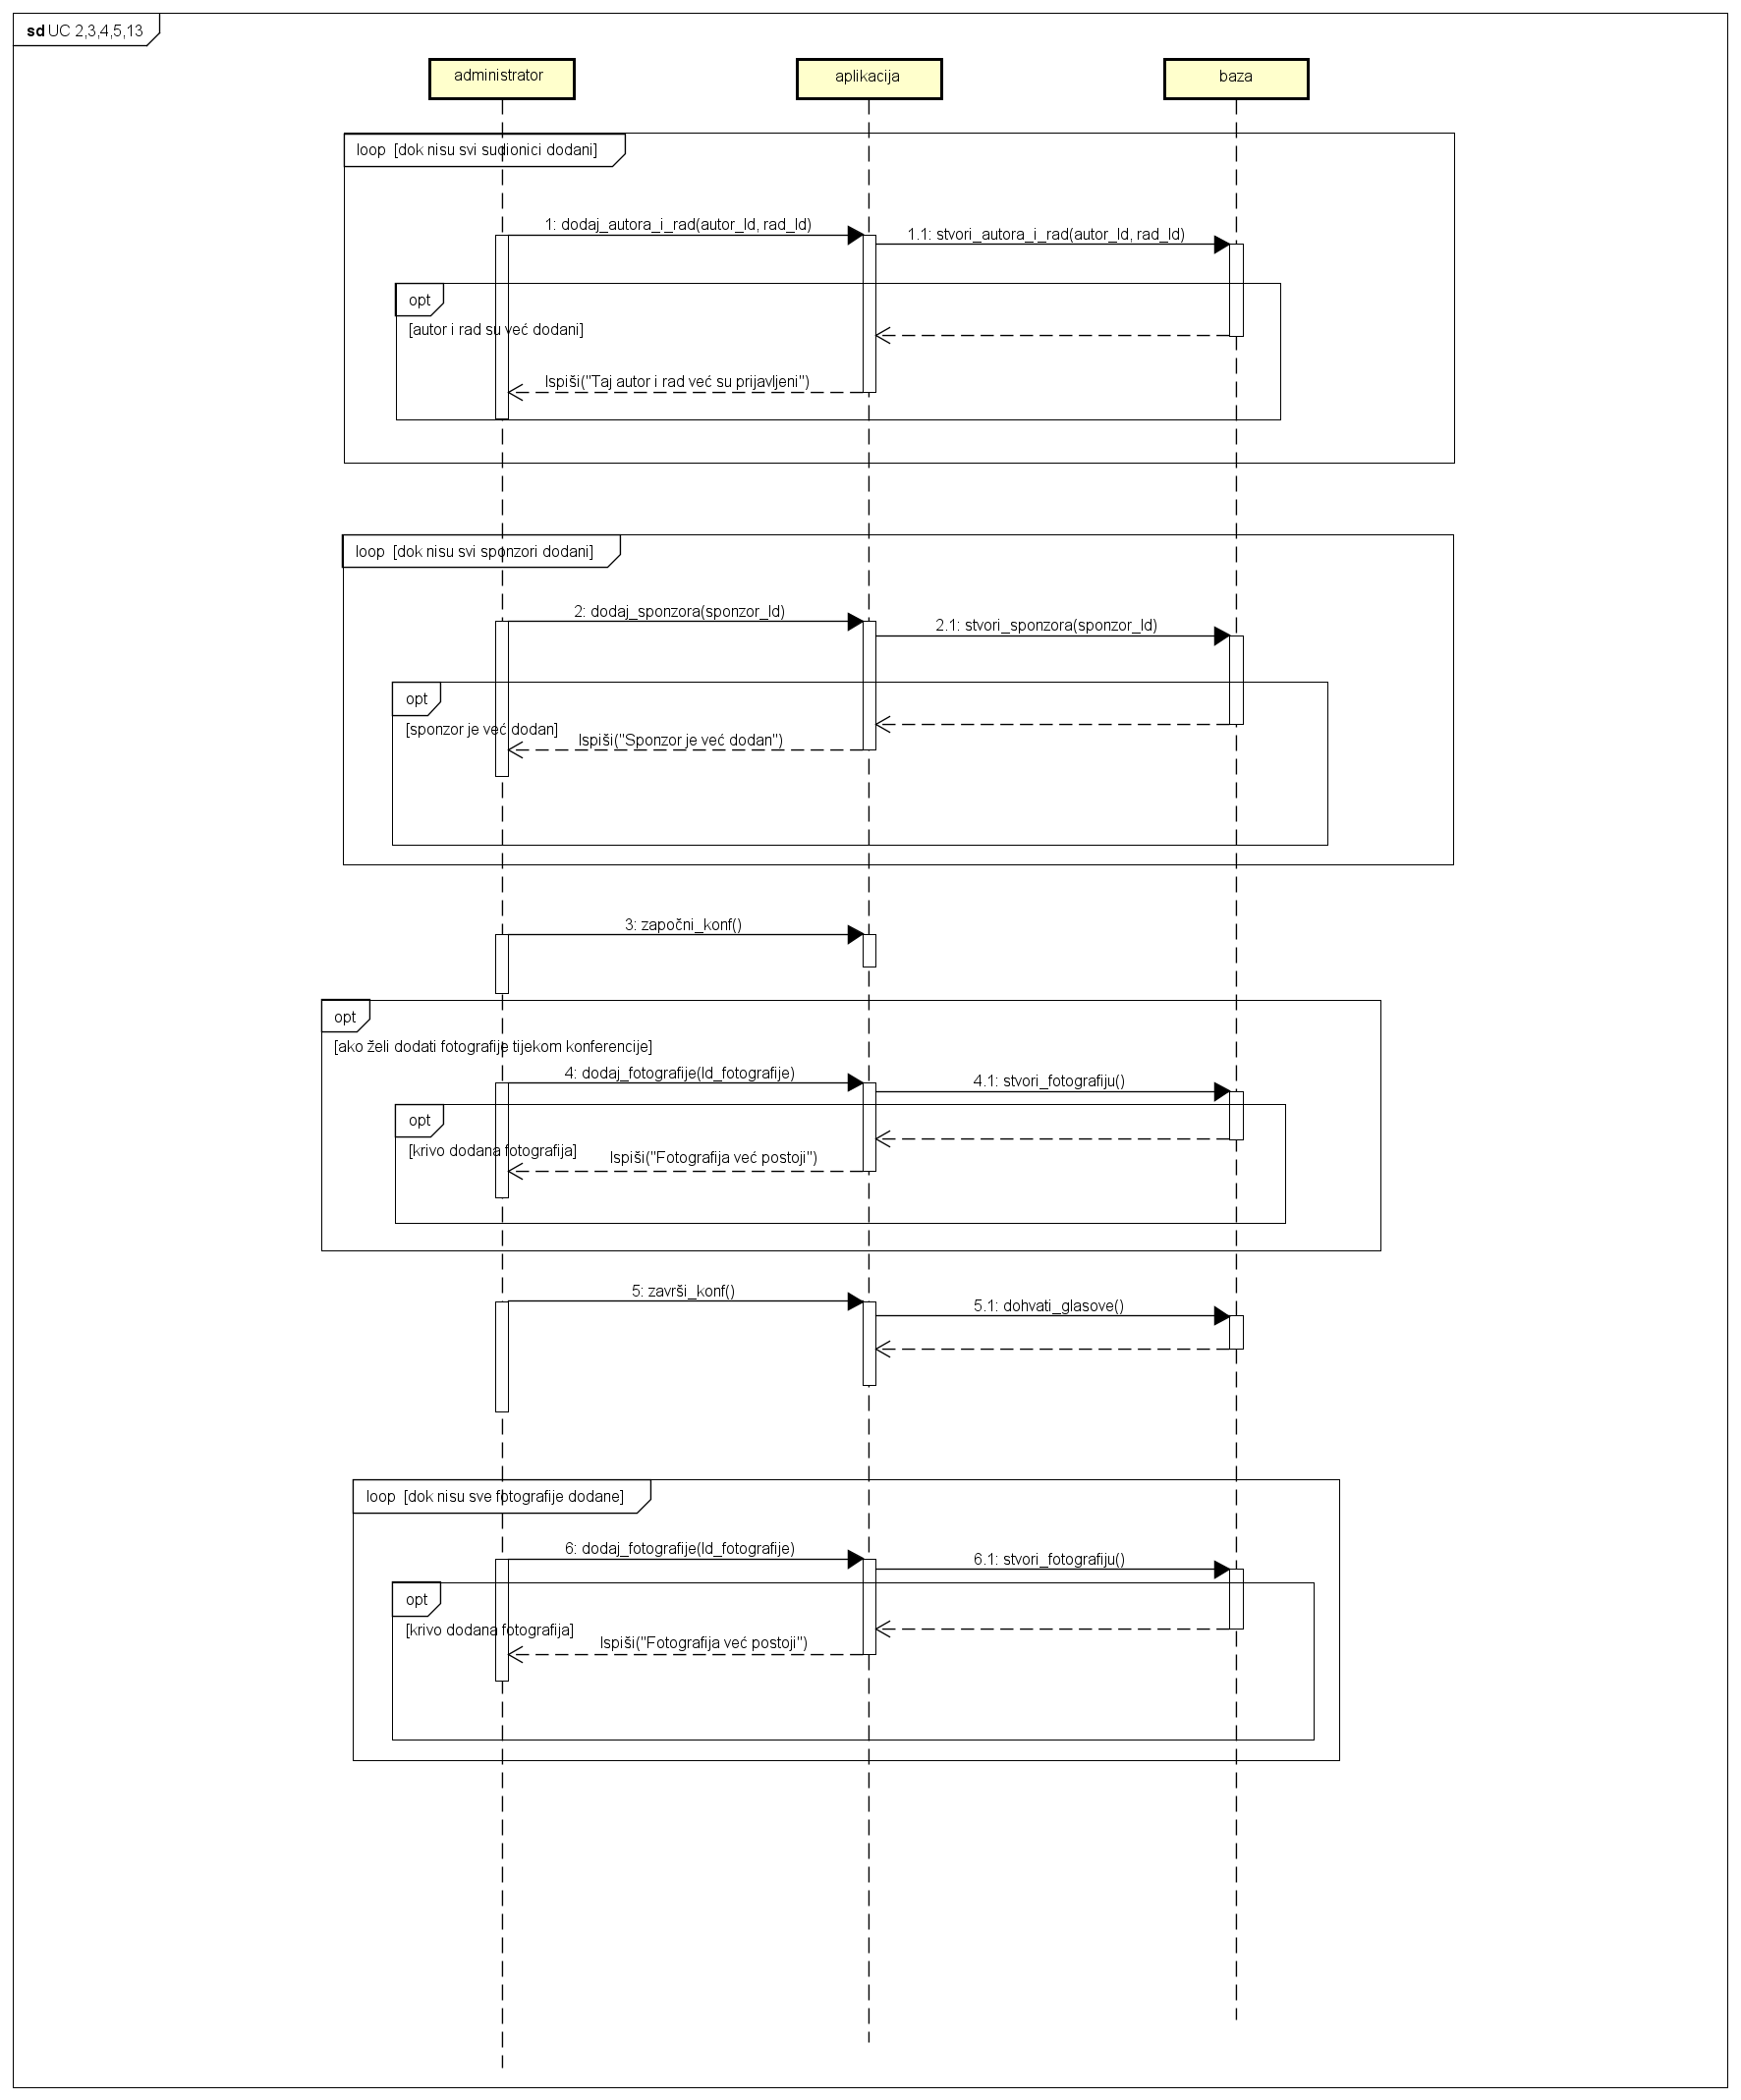
\includegraphics[scale=0.3]{dijagrami/sekv2.png}%veličina slike u odnosu na originalnu datoteku i pozicija slike
					\centering
					\caption{Sekvencijski dijagram korištenja aplikacije od strane administratora}
					\label{fig:promjene10}
				\end{figure}
				\eject
	
		\section{Ostali zahtjevi}
		
%			\textbf{\textit{dio 1. revizije}}\\
		 
			 \begin{packed_item}
				\item Sustav mora omogućiti istovremeni rad više korisnika u stvarnom vremenu
				\item Sustav i korisničko sučelje moraju podržavati znakovlje hrvatske abecede (dijakritičke znakove) prilikom prikazivanja tekstualnog sadržaja te unosa
				\item Pristupanje bazi podataka, tj. izvršavanje dijela programa u kojem se pristupa bazi podataka ne smije trajati duže od nekoliko sekundi
				\item Sustav treba biti implementiran kao web aplikacija koristeći objektno - orijentirane jezike
				\item Neispravnim korištenjem korisničkog sučelja, ne smije se narušiti funkcionalnost i rad sustava
				\item Sustav treba biti jednostavan i intuitivan za korištenje, odnosno korisnik ga mora moći koristiti bez korištenja (opširnih) uputa
				\item Prilikom nadogradnje sustava, ne smiju biti narušene njegove postojeće funkcionalnosti
				\item Veza s bazom podataka mora biti dobro zaštićena, brza i otporna na vanjske greške
				\item Sustav je responzivan na mobilnim uređajima
				\item Pristup sustavu treba biti omogućen iz javne mreže preko HTTPS protokola
			\end{packed_item}
			 
			 
			 
	
	\chapter{Arhitektura i dizajn sustava}
		
		Na arhitekturu sustava najveći utjecaj imali su principi oblikovanja: Podijeli pa vladaj, Zadrži razinu apstrakcije te Oblikuj za prenosivost. Princip Podijeli pa vladaj očituje se u podijeli sustava na manje komponente radi povećane razumljivosti te lakše zamjene dijelova i ponovnog korištenja. Princip Zadrži razinu apstrakcije omogućava razumijevanje poante podsustava bez poznavanja nepotrebnih detalja. Korištenje Jave kao objektno orijentiranog programskog jezika omogućuje nam upotrebu razreda, podatkovnih apstrakcija koje sadrže proceduralne apstrakcije (metode). Osim upotrebe razreda Java omogućuje rad na više platformi, čime je osigurana prenosivost.
		
	Organizacija sustava s najviše razine apstrakcije je klijent-poslužitelj-baza podataka. Klijenta predstavlja preglednik weba koji omogućuje korisniku slanje zahtjeva poslužitelju protokolom HTTP \textit{(engl. Hyper Text Transfer Protocol)}. Poslužitelj je server koji poslužuje te zahtjeve, prosljeđuje ih web aplikaciji koja se pokreće preko poslužitelja te vraća odgovore koji se prikazuju preko klijenta (preglednika). Podaci su spremljeni u bazi podataka te joj po potrebi pristupa web aplikacija koristeći SQL upite.
					\begin{figure}[H]
						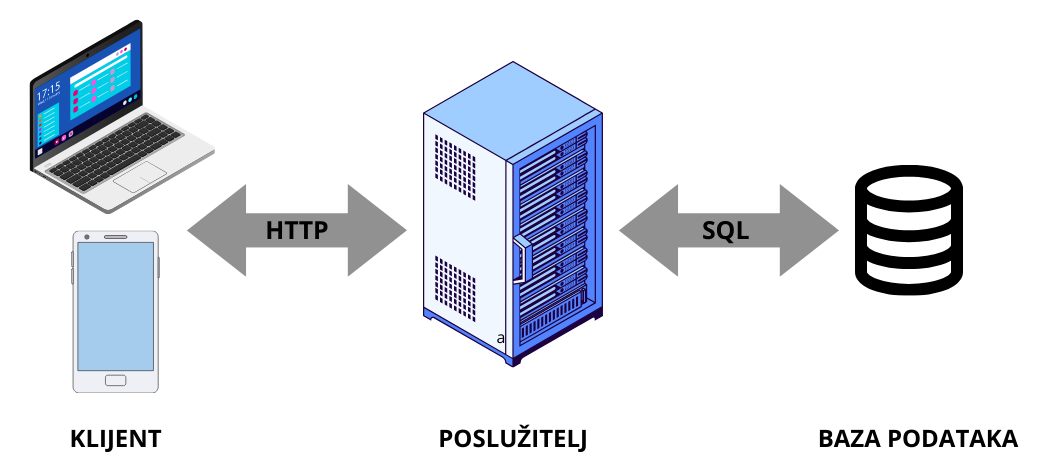
\includegraphics[scale=0.4]{slike/arh1.PNG} %veličina slike u odnosu na originalnu datoteku i pozicija slike
						\centering
						\caption{Organizacija sustava s najviše razine apstrakcije}
						\label{fig:promjene4}
					\end{figure}	
	Arhitektura aplikacije je troslojna. Prvi sloj je \textbf {kontroler} koji prima zahtjeve, poziva odgovarajuće metode drugog sloja \textbf {servisa}, te na kraju vraća odgovore. Servis sadrži poslovnu logiku aplikacije, a za pristup podacima koristi treći sloj \textbf {repozitorij} koji komunicira s bazom podataka.
					\begin{figure}[H]
						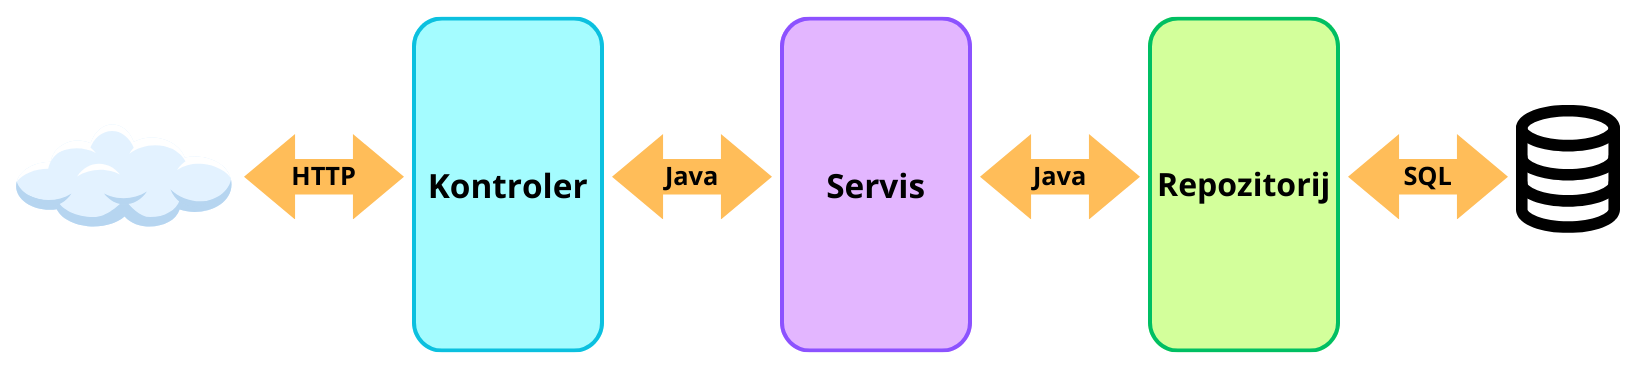
\includegraphics[scale=0.3]{slike/arh2.PNG} %veličina slike u odnosu na originalnu datoteku i pozicija slike
						\centering
						\caption{Organizacija aplikacije}
						\label{fig:promjene5}
					\end{figure}	
	Za izradu naše aplikacije korišten je Java Spring Boot okvir koji koristi MVC \textit{(engl. Model-View-Controller)} oblikovni obrazac u kojem je poslužitelj organiziran u tri dijela u cilju razdvajanja nadležnosti. \textbf {Kontroler} prima zahtjeve koje prosljeđuje modelu te upravlja modelom i pogledom. \textbf {Model} je zadužen za obradu i dohvat podataka te komunicira s bazom podataka. \textbf {Pogled} prezentira dostavljene podatke.
	
		

		

				
		\section{Baza podataka}
		U aplikaciji će baza podataka bit prikazana relacijskim modelom podataka. Objekti relacijskog modela su relacije, a svaka ima jedinstveno ime unutar sheme baze podataka. Relacija je tablica čiji se imenovani stupci nazivaju atributi, a redci n-torke. Ključ entiteta je skup atributa koji jednoznačno određuje entitet. U našem sustavu entiteti baze podataka su:
	\begin{itemize}
		\item Rad
		\item Osoba
		\item Konferencija
		\item Prisutan\_na
		\item Mjesto
		\item Fotografija
		\item Pokrovitelj	
		\item Pokrovitelj\_na
		\item Password\_token	
	\end{itemize}
			\subsection{Opis tablica}
			Entitet \textbf {Rad} sadrži sve važne informacije o radu. Sadrži atribute: ID rada, naziv postera, naziv prezentacije, naslov rada, ID autora, ID konferencije na koju je prijavljen, osvojeni plasman, url postera i prezentacije i ukupan broj osvojenih glasova na toj konferenciji. Atributi naziv prezentacije, url prezentacije i plasman su opcionalni te stoga mogu poprimiti vrijednost null. Entitet Rad u binarnoj je vezi \textit{(Many-to-One)} s entitetom Konferencija i u vezi \textit{(Many-to-One)} s entitetom Osoba.
				\begin{longtblr}[
					label=none,
					entry=none
					]{
						width = \textwidth,
						colspec={|X[7,l]|X[6, l]|X[20, l]|}, 
						rowhead = 1,
					} %definicija širine tablice, širine stupaca, poravnanje i broja redaka naslova tablice
					\hline \SetCell[c=3]{c}{\textbf{Rad}}	 \\ \hline[3pt]
					\SetCell{LightGreen}id & SERIAL	&  	jedinstveni identifikator rada 	\\ \hline
					nazivPoster	& VARCHAR &   	naziv postera koji prikazuje rad\\ \hline 
					nazivPptx & VARCHAR &   naziv prezentacije koja prikazuje rad, može biti null\\ \hline 
					naslov & VARCHAR	&    naslov rada\\ \hline 
					ukupnoGlasova & INT &   ukupan broj osvojenih glasova na konferenciji\\ \hline 
					urlPoster	& VARCHAR &   	url postera koji prikazuje rad\\ \hline 
					urlPptx & VARCHAR &   url prezentacije koja prikazuje rad, može biti null\\ \hline 
					plasman & INT &   plasman na konferenciji, može biti null\\ \hline 
					\SetCell{LightBlue}idKonf	& SERIAL &   	jedinstveni identifikator konferencije\\ \hline 
					\SetCell{LightBlue}idAutor & SERIAL&    jedinstveni identifikator autora\\ \hline 
				\end{longtblr}						
			
			\noindent Entitet \textbf {Osoba} sadrži informacije o autorima, korisnicima te adminima. Sadrži atribute: ID osobe, email, ime i prezime, lozinka (u slučaju da se radi o autoru koji ujedno nije i korisnik bit će null) i uloga koji može poprimiti vrijednosti "admin", "korisnik" ili "autor". Entitet Osoba u binarnoj je vezi s entitetom Rad \textit{(One-to-Many)}, s entitetom Konferencija \textit{(One-to-Many)}, s entitetom Konferencija \textit{(Many-to-Many)} i s entitetom Paassword\_token \textit{(One-to-One)}.
				\begin{longtblr}[
					label=none,
					entry=none
					]{
						width = \textwidth,
						colspec={|X[7,l]|X[6, l]|X[20, l]|}, 
						rowhead = 1,
					} %definicija širine tablice, širine stupaca, poravnanje i broja redaka naslova tablice
					\hline \SetCell[c=3]{c}{\textbf{Osoba}}	 \\ \hline[3pt]
					\SetCell{LightGreen}id & SERIAL	&  	jedinstveni identifikator osobe\\ \hline
					email	& VARCHAR &   	email osobe\\ \hline 
					ime & VARCHAR &   ime osobe\\ \hline 
					prezime & VARCHAR	&    prezime osobe\\ \hline 
					lozinka & VARCHAR &   hash lozinke korisnika ili admina\\ \hline 
					uloga & VARCHAR &  uloga osobe\\ \hline 
				\end{longtblr}		

			\noindent Entitet \textbf {Konferencija} sadrži informacije o stručnoj konferenciji koja će se održati. Sadrži atribute: ID konferencije, poveznica na video prijenos konferencije, pin za ulazak na konferenciju, vrijeme početka i vrijeme kraja konferencije, ID admina zaduženog za konferenciju i adresu i poštanski broj mjesta u kojem se održava konferencija. Entitet Konferencija u binarnoj je vezi s entitetom Rad \textit{(One-to-Many)}, u binarnoj vezi \textit{(Many-to-One)} i \textit{(Many-to-Many)} s entitetom Osoba, u vezi \textit{(Many-to-One)} s entitetom Mjesto, \textit{(One-to-Many)} s entitetom Fotografija i \textit{(Many-to-Many)} s entitetom Pokrovitelj.
				\begin{longtblr}[
					label=none,
					entry=none
					]{
						width = \textwidth,
						colspec={|X[6,l]|X[6, l]|X[20, l]|}, 
						rowhead = 1,
					} %definicija širine tablice, širine stupaca, poravnanje i broja redaka naslova tablice
					\hline \SetCell[c=3]{c}{\textbf{Konferencija}}	 \\ \hline[3pt]
					\SetCell{LightGreen}id & SERIAL	&  	jedinstveni identifikator konferencije \\ \hline
					urlVideo	& VARCHAR &   	 poveznica na direktno video praćenje
trenutnih događanja u glavnoj konferencijskoj dvorani\\ \hline 
					pin & INT &   jedinstveni pin konferencije\\ \hline 
					vrijemePocetak & TIMESTAMP	&    početak konferencije\\ \hline 
					vrijemeKraj & TIMESTAMP	&    kraj konferencije\\ \hline 
					adresa	& VARCHAR &   	 adresa konferencije\\ \hline 
					\SetCell{LightBlue} idAdmin & SERIAL &   jedinstveni identifikator admina zaduženog za konferenciju\\ \hline 
					\SetCell{LightBlue} pbr & INT &   poštanski broj mjesta u kojem se održava konferencija\\ \hline 
				\end{longtblr}		

			\noindent Entitet \textbf {Prisutan\_na} sadrži informacije o prisutnosti pojedinog korisnika na određenoj konferenciji te je li glasao na njoj ili ne. Sadrži atribute: ID konferencije, ID korisnika i glasao. Entitet Prisutan\_na rezultat je binarne veze \textit{(Many-to-Many)} entiteta Osoba s entitetom Konferencija.
				\begin{longtblr}[
					label=none,
					entry=none
					]{
						width = \textwidth,
						colspec={|X[6,l]|X[6, l]|X[20, l]|}, 
						rowhead = 1,
					} %definicija širine tablice, širine stupaca, poravnanje i broja redaka naslova tablice
					\hline \SetCell[c=3]{c}{\textbf{Prisutan\_na}}	 \\ \hline[3pt]
					\SetCell{LightGreen}idKonf & SERIAL	&  	jedinstveni identifikator konferencije \\ \hline
					\SetCell{LightGreen}idKorisnik	& SERIAL &   	jedinstveni identifikator korisnika\\ \hline 
					glasao & BOOLEAN &   informacija je li korisnik već glasao na konferenciji\\ \hline 
				\end{longtblr}

			\noindent Entitet \textbf {Mjesto} sadrži informacije o pojedinom mjestu. Sadrži atribute: poštanski broj i naziv mjesta. Entitet Mjesto u binarnoj je vezi s entitetom Konferencija \textit{(One-to-Many)}. 
				\begin{longtblr}[
					label=none,
					entry=none
					]{
						width = \textwidth,
						colspec={|X[6,l]|X[6, l]|X[20, l]|}, 
						rowhead = 1,
					} %definicija širine tablice, širine stupaca, poravnanje i broja redaka naslova tablice
					\hline \SetCell[c=3]{c}{\textbf{Mjesto}}	 \\ \hline[3pt]
					\SetCell{LightGreen}pbr & INT &   poštanski broj mjesta \\ \hline
					naziv	& VARCHAR &   	naziv mjesta\\ \hline 
				\end{longtblr}

			\noindent Entitet \textbf {Fotografija} sadrži informacije o uslikanoj fotografiji te na kojoj konferenciji je uslikana. Sadrži atribute: ID fotografije, url fotografije i ID konferencije. Entitet Fotografija u binarnoj je vezi s entitetom Konferencija \textit{(Many-to-One)}. 
				\begin{longtblr}[
					label=none,
					entry=none
					]{
						width = \textwidth,
						colspec={|X[6,l]|X[6, l]|X[20, l]|}, 
						rowhead = 1,
					} %definicija širine tablice, širine stupaca, poravnanje i broja redaka naslova tablice
					\hline \SetCell[c=3]{c}{\textbf{Fotografija}}	 \\ \hline[3pt]
					\SetCell{LightGreen}id & SERIAL	&  	jedinstveni identifikator fotografije\\ \hline
					urlSlike	& VARCHAR &   	url fotografije\\ \hline 
					\SetCell{LightBlue}idKonf & SERIAL &   jedinstveni identifikator konferencije\\ \hline 
				\end{longtblr}

			\noindent Entitet \textbf {Pokrovitelj} sadrži informacije o pokrovitelju. Sadrži atribute: ID pokrovitelja,  url stranice pokrovitelja, naziv pokrovitelja i url slike. Entitet Pokrovitelj u binarnoj je vezi s entitetom Konferencija \textit{(Many-to-Many)}. 
				\begin{longtblr}[
					label=none,
					entry=none
					]{
						width = \textwidth,
						colspec={|X[7,l]|X[6, l]|X[20, l]|}, 
						rowhead = 1,
					} %definicija širine tablice, širine stupaca, poravnanje i broja redaka naslova tablice
					\hline \SetCell[c=3]{c}{\textbf{Pokrovitelj}}	 \\ \hline[3pt]
					\SetCell{LightGreen}id & SERIAL	&  	jedinstveni identifikator pokrovitelja\\ \hline
					url	& VARCHAR &   	poveznica na stranicu pokrovitelja\\ \hline 
					naziv	& VARCHAR &   	naziv pokrovitelja\\ \hline 
					urlSlike	& VARCHAR &   	logo pokrovitelja\\ \hline
				\end{longtblr}

			\noindent Entitet \textbf {Pokrovitelj\_na} sadrži informacije o uključenosti pokrovitelja na pojedinoj konferenciji. Sadrži atribute: ID konferencije i ID pokrovitelja. Entitet Pokrovitelj\_na rezultat je binarne veze \textit{(Many-to-Many)} entiteta Pokrovitelj i Konferencija.
				\begin{longtblr}[
					label=none,
					entry=none
					]{
						width = \textwidth,
						colspec={|X[6,l]|X[6, l]|X[20, l]|}, 
						rowhead = 1,
					} %definicija širine tablice, širine stupaca, poravnanje i broja redaka naslova tablice
					\hline \SetCell[c=3]{c}{\textbf{Pokrovitelj\_na}}	 \\ \hline[3pt]
					\SetCell{LightGreen}idKonf & SERIAL	&  	jedinstveni identifikator konferencije \\ \hline
					\SetCell{LightGreen}idPokrovitelj	& SERIAL &   	jedinstveni identifikator pokrovitelja\\ \hline 
				\end{longtblr}
			\noindent Entitet \textbf {Password\_token} sadrži informacije o tokenu koji je pojedina osoba dobila kada je zatražila promjenu lozinke. Sadrži atribute: ID tokena, istek tokena, token i ID osobe čiji je token. Entitet Password\_token u binarnoj je vezi s entitetom Osoba \textit{(One-to-One)}. .
				\begin{longtblr}[
					label=none,
					entry=none
					]{
						width = \textwidth,
						colspec={|X[6,l]|X[6, l]|X[20, l]|}, 
						rowhead = 1,
					} %definicija širine tablice, širine stupaca, poravnanje i broja redaka naslova tablice
					\hline \SetCell[c=3]{c}{\textbf{Pokrovitelj\_na}}	 \\ \hline[3pt]
					\SetCell{LightGreen}id & SERIAL	&  	jedinstveni identifikator tokena \\ \hline
					istek	& DATE &   	datum isteka tokena\\ \hline 
					token	& VARCHAR &   	token\\ \hline 
					\SetCell{LightBlue}idOsoba & SERIAL &   jedinstveni identifikator osobe\\ \hline 
				\end{longtblr}
			\subsection{Dijagram baze podataka}
%				\textit{ U ovom potpoglavlju potrebno je umetnuti dijagram baze podataka. Primarni i strani ključevi moraju biti označeni, a tablice povezane. Bazu podataka je potrebno normalizirati. Podsjetite se kolegija "Baze podataka".}
					\begin{figure}[H]
						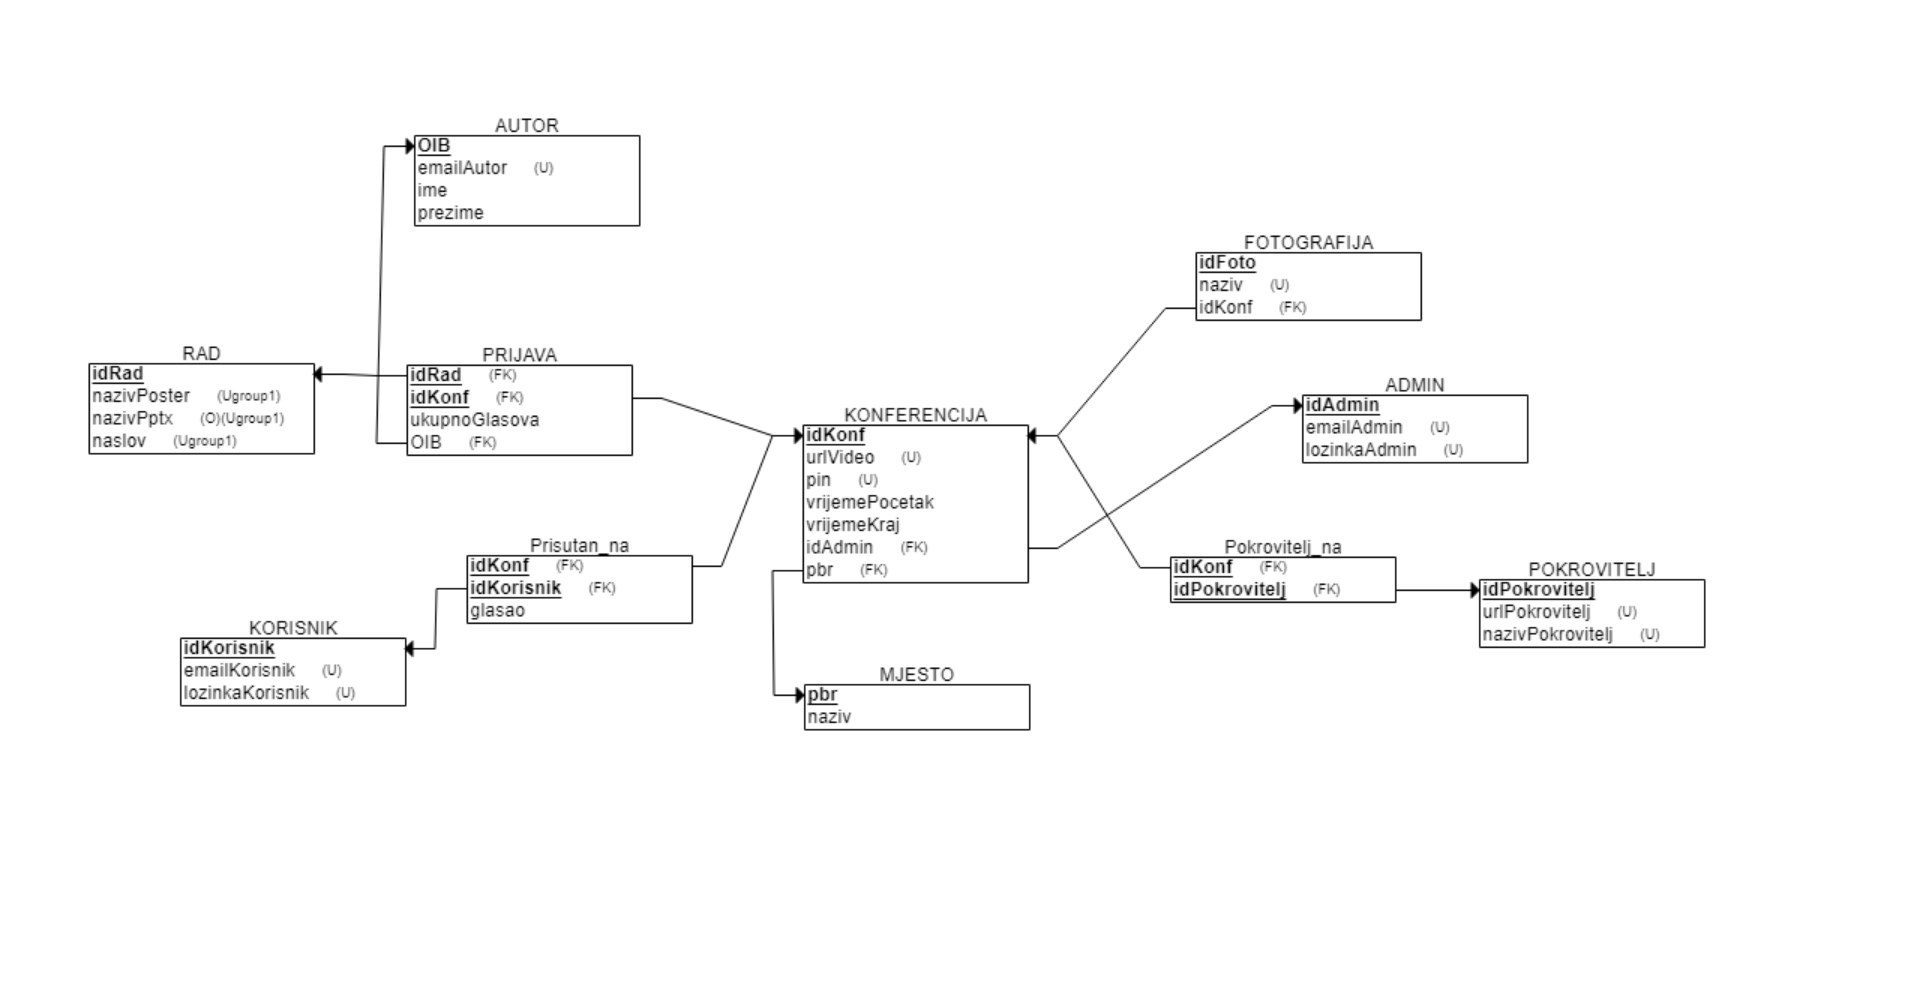
\includegraphics[scale=0.55]{dijagrami/dijagram baze podataka.PNG} %veličina slike u odnosu na originalnu datoteku i pozicija slike
						\centering
						\caption{Dijagram baze podataka}
						\label{fig:promjene3}
					\end{figure}			
			\eject
			
			
		\section{Dijagram razreda}
		
		
			Radi preglednosti, dijagram je razlomljen na nekoliko dijelova. Na njima su prikazani razredi koji pripadaju backend dijelu MVC arhitekture.
			Na slici 4.4 je prikazan Model dio. Model klase služe za prijenos podataka između baze podataka i serverske strane aplikacije. Ti su objekti zapravo preslika baze podataka, ali umjesto relacijske koristimo objektno-orijentiranu paradigmu. 
			Razred Konferencija predstavlja konferenciju koja se prikazuje u aplikaciji. 
Razred Mjesto predstavlja lokaciju na kojoj se konferencija održava.
Razred Osoba predstavlja čovjeka koji na neki način sudjeluje na konferenciji.  Taj razred ima atribut uloga kojim se određuje je li ta osoba autor, administrator ili posjetitelj konferencije. 
Razred Rad predstavlja rad (poster i/ili pptx) kojim se autor predstavlja na konferenciji.
Razred PrisutanNa omogućuje da pratimo tko je na konferenciji te da li je ta osoba glasala za neki rad.
Razred Fotografija predstavlja fotografije konferencije koje administrator stavlja u aplikaciju tijekom ili nakon konferencije.
Razred Pokrovitelj predstavlja sponzore konferencije. 
Razred PasswordToken omogućuje postavljanje i promjenu lozinku.
Razred Media omogućuje lakši prikaz i pohranu medijskih sadržaja.

			\begin{figure}[H]
				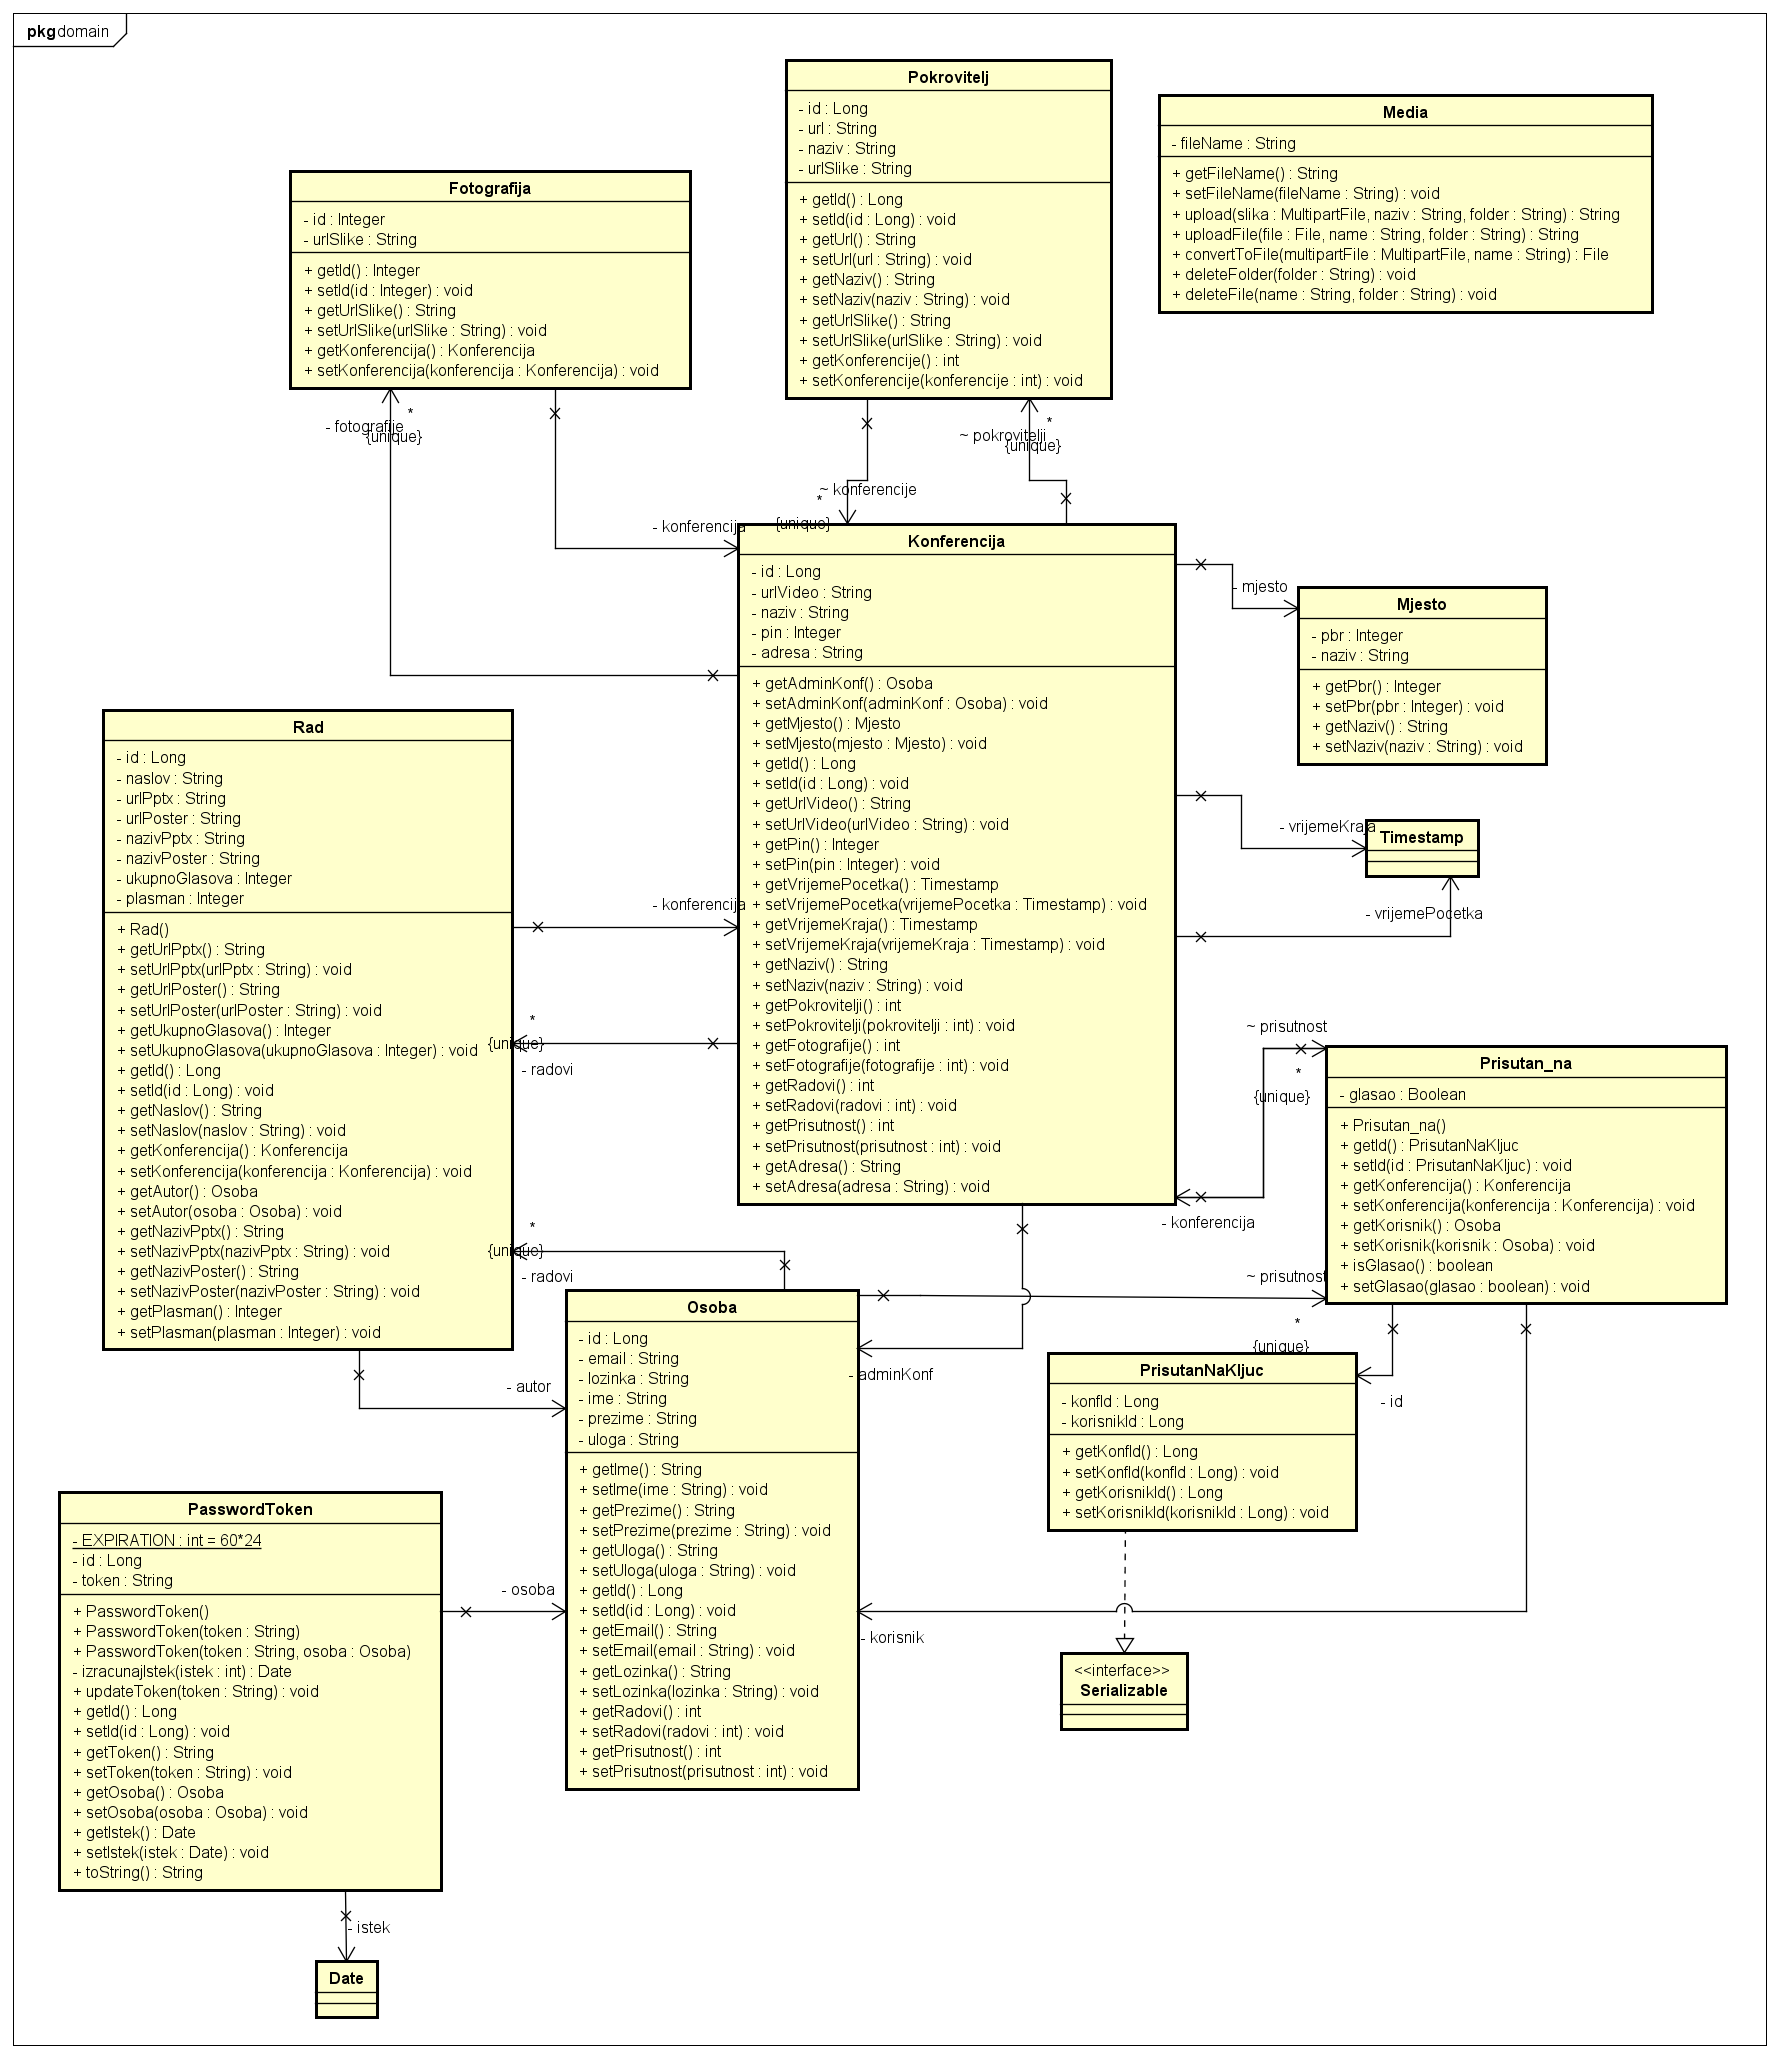
\includegraphics[scale=0.35]{dijagrami/models.png}%veličina slike u odnosu na originalnu datoteku i pozicija slike
				\centering
				\caption{Dijagram razreda - dio Models}
				\label{fig:promjena9}
			\end{figure}
			

			Na slikama 4.5, 4.6, 4.7 i 4.8 je prikazan glavni dijagram u čijem središtu se nalazi JPARepository o kojem ovise ostala sučelja koja su specifična za svaki objekt. Ova sučelja nam omogućuju da izbjegnemo pisanje složenih SQL upita i umjesto toga koristimo generičke metode za izvođenje uobičajenih operacija s bazom podataka.
U dijagramu su i servisi u kojima su funkcije za obradu podataka. Po potrebi zovu repozitorijeve funkcije kako bi došli do baze podataka.
Kontroleri nam služe za komunikaciju s frontendom. 
U klasi PosterizedApplication se nalazi glavna funkcija za pokretanje aplikacije. WebSecurityBasic je zadužen za zaštitu cijele aplikacije.

			

			\begin{figure}[H]
				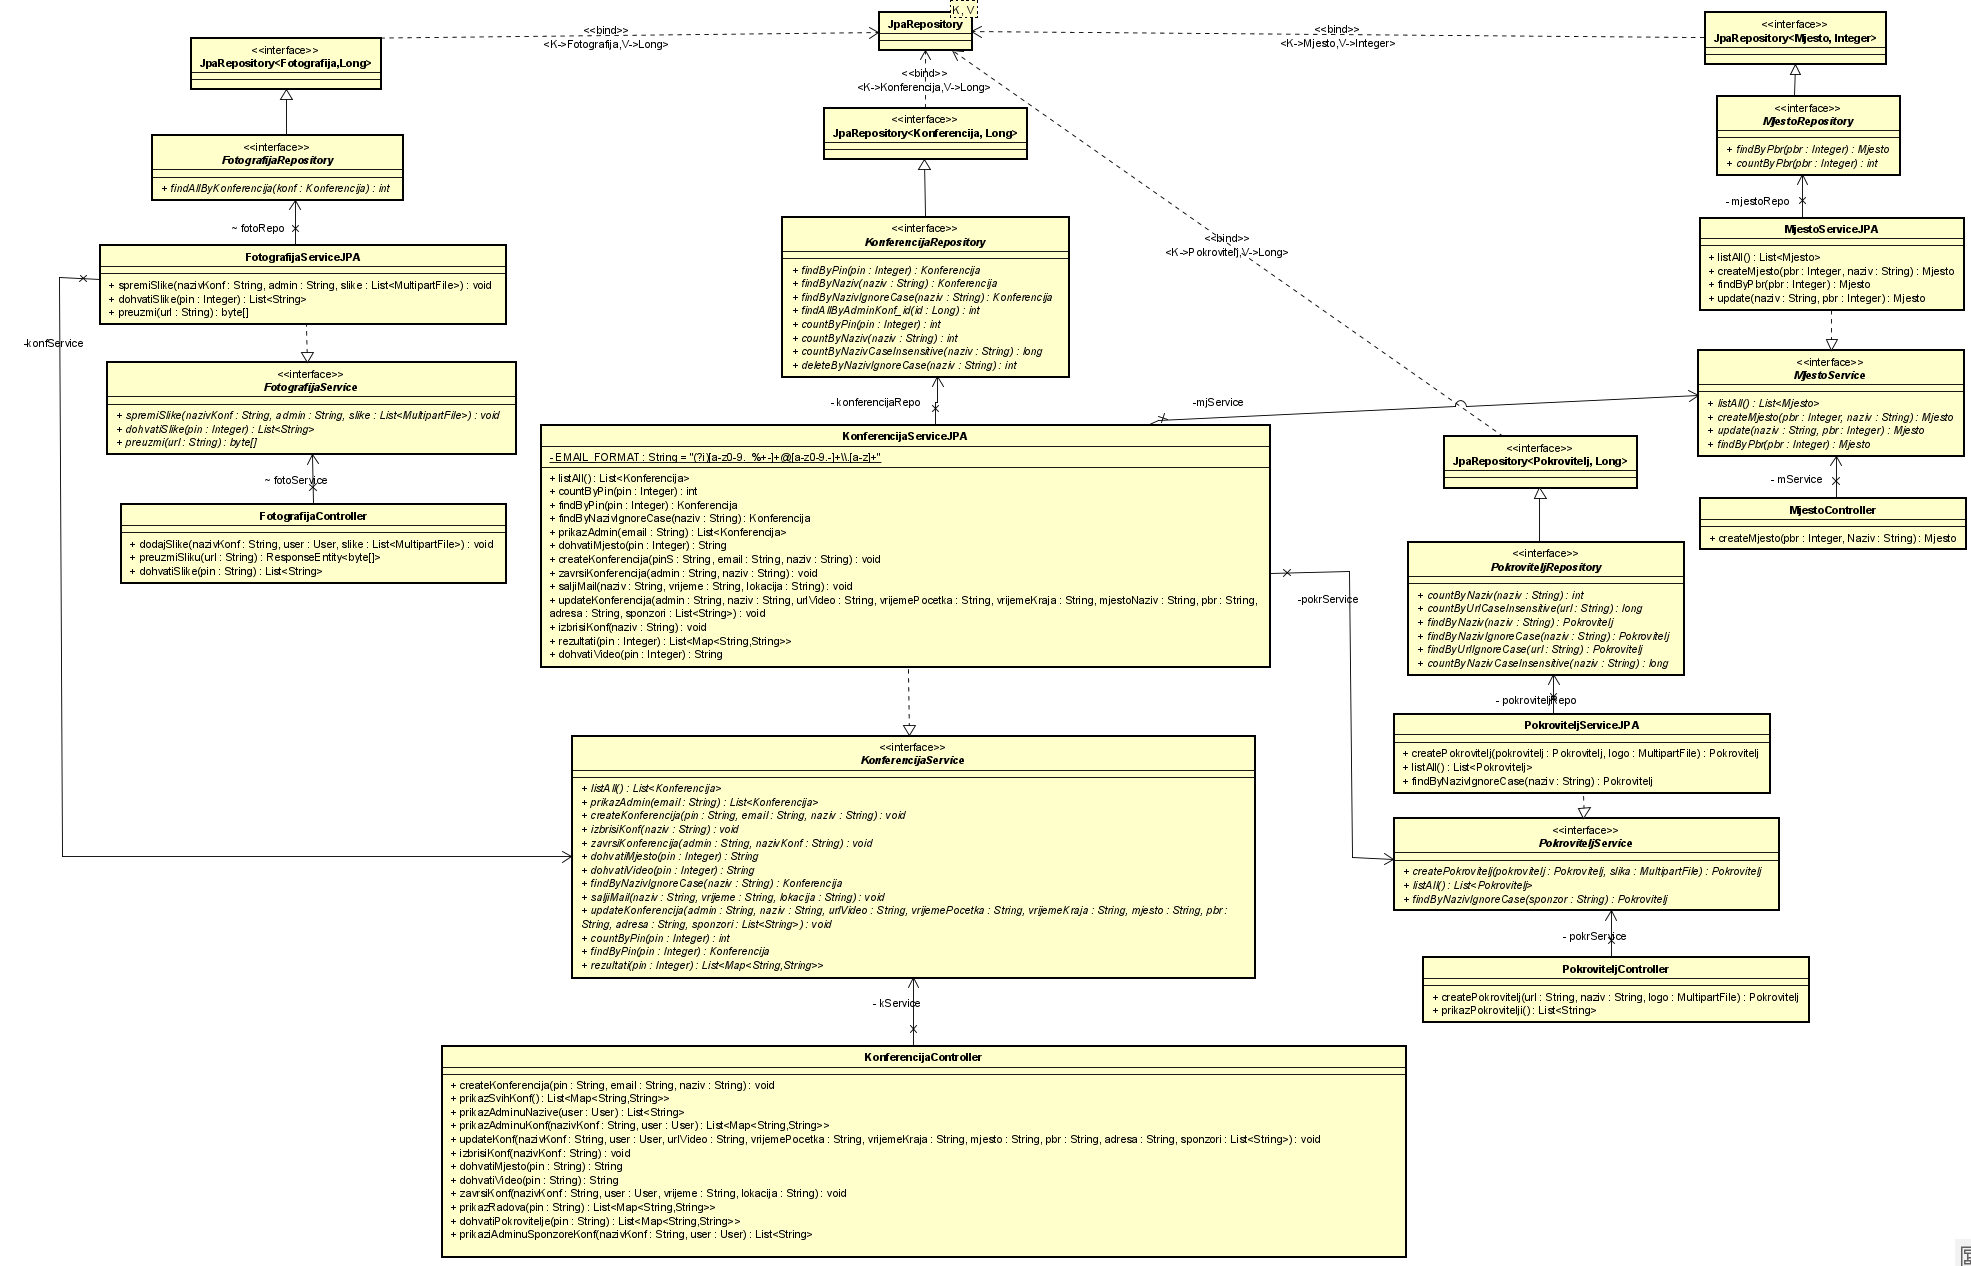
\includegraphics[scale=0.15]{dijagrami/glavni_1.png}%veličina slike u odnosu na originalnu datoteku i pozicija slike
				\centering
				\caption{Dijagram razreda - glavni dijagram 1.dio}
				\label{fig:promjena9.1}
			\end{figure}
			
			\begin{figure}[H]
				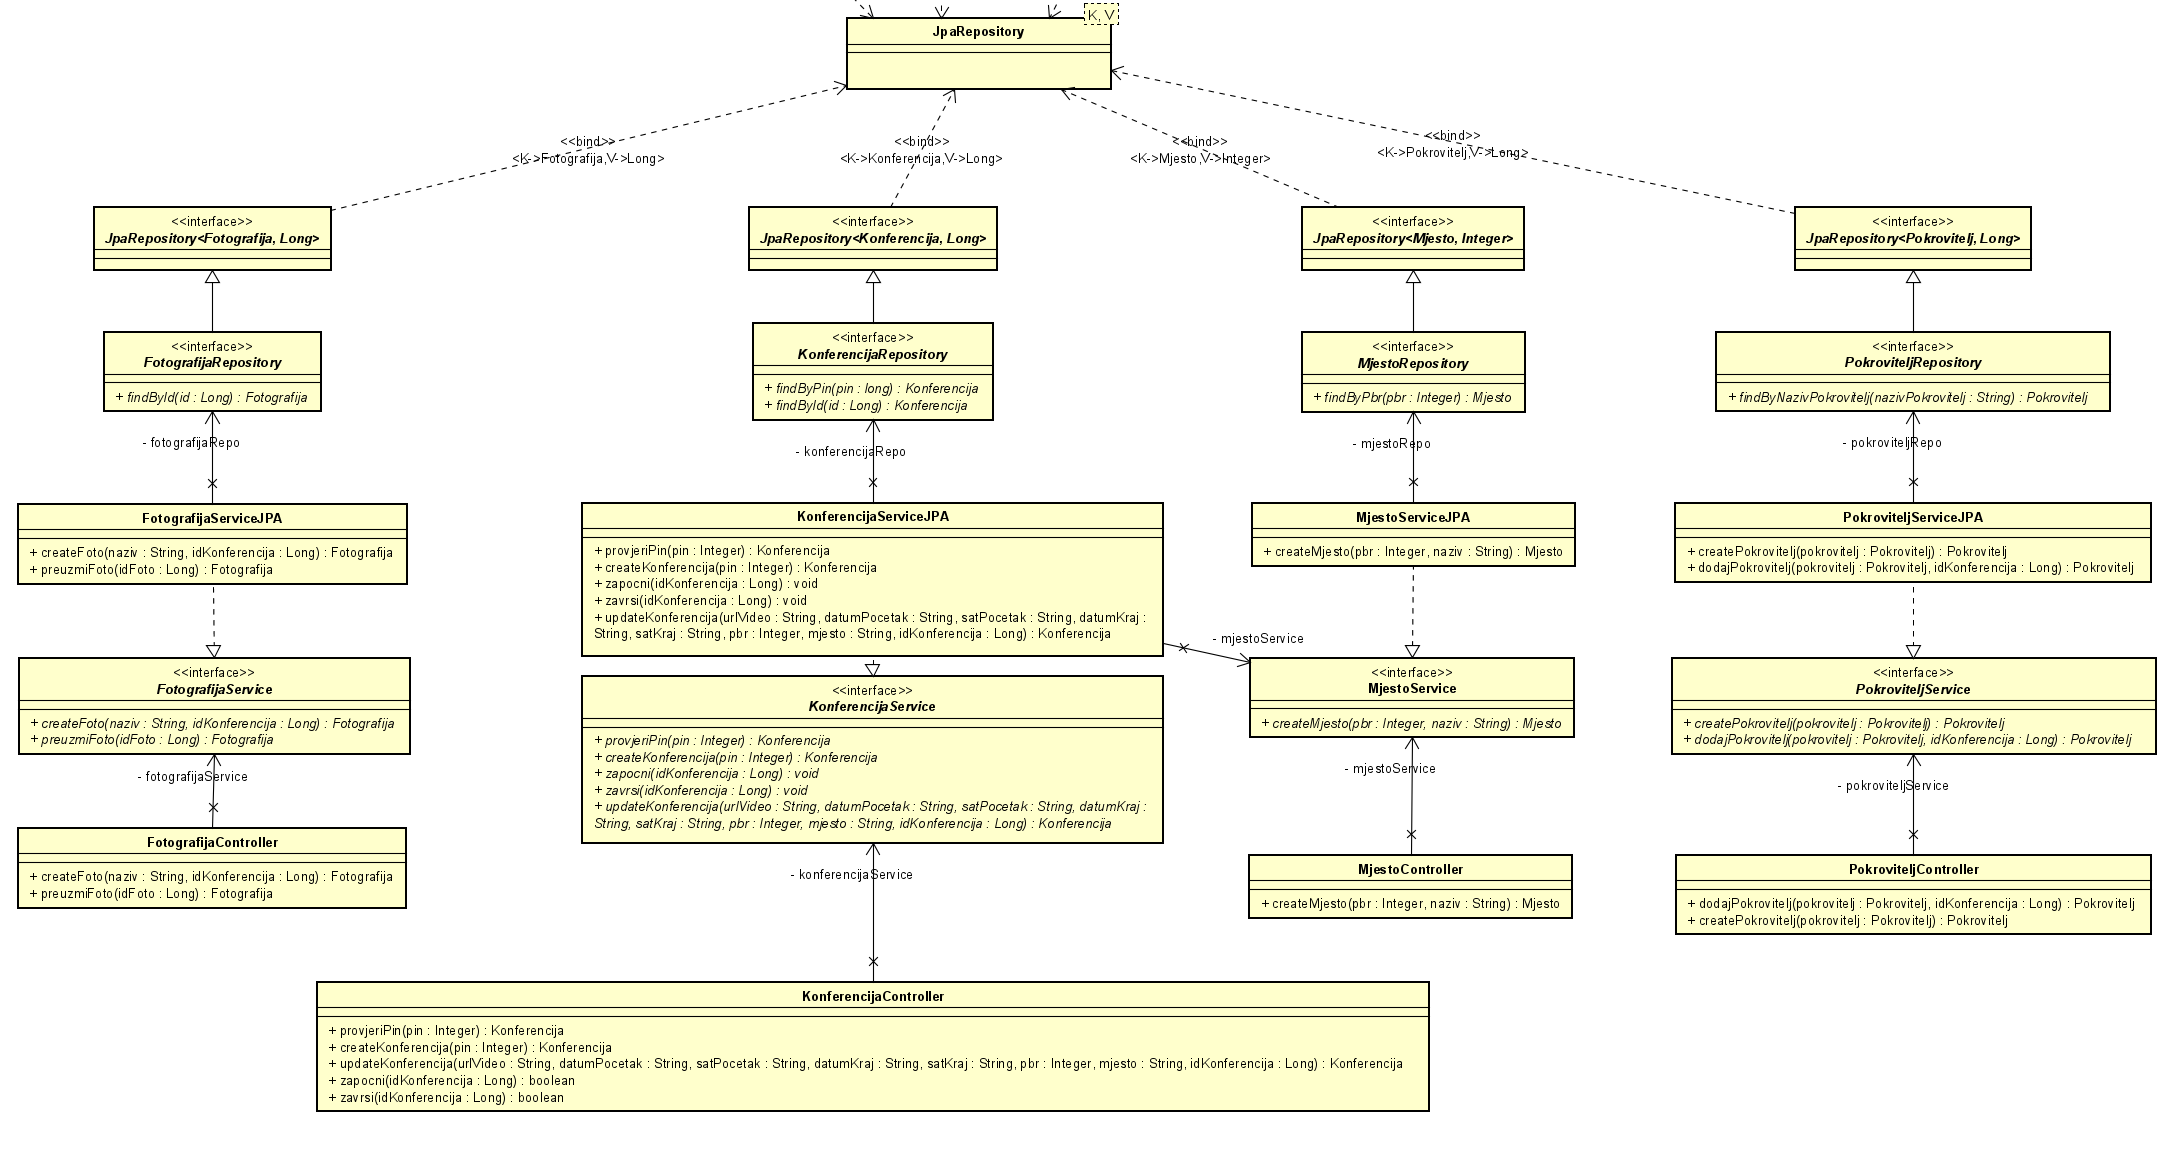
\includegraphics[scale=0.13]{dijagrami/glavni_2.png}%veličina slike u odnosu na originalnu datoteku i pozicija slike
				\centering
				\caption{Dijagram razreda - glavni dijagram 2.dio}
				\label{fig:promjena9.2}
			\end{figure}
			
			\begin{figure}[H]
				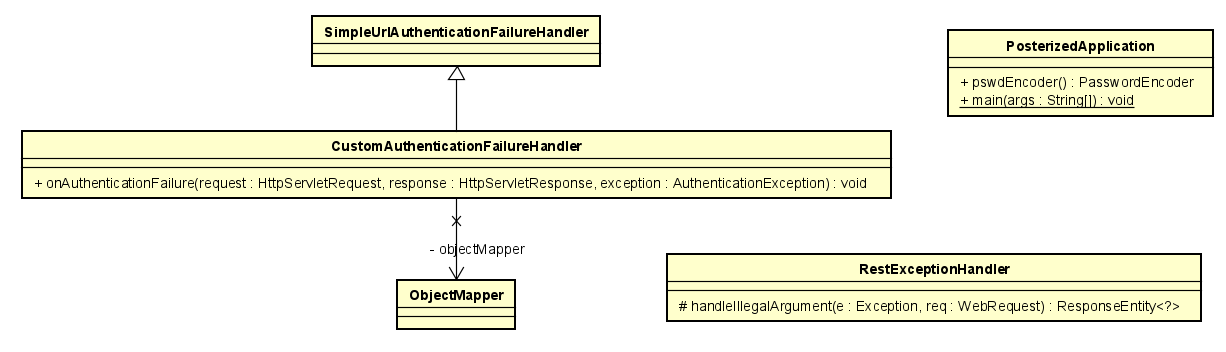
\includegraphics[scale=0.15]{dijagrami/glavni_3.png}%veličina slike u odnosu na originalnu datoteku i pozicija slike
				\centering
				\caption{Dijagram razreda - glavni dijagram 3.dio}
				\label{fig:promjena9.3}
			\end{figure}

			\begin{figure}[H]
				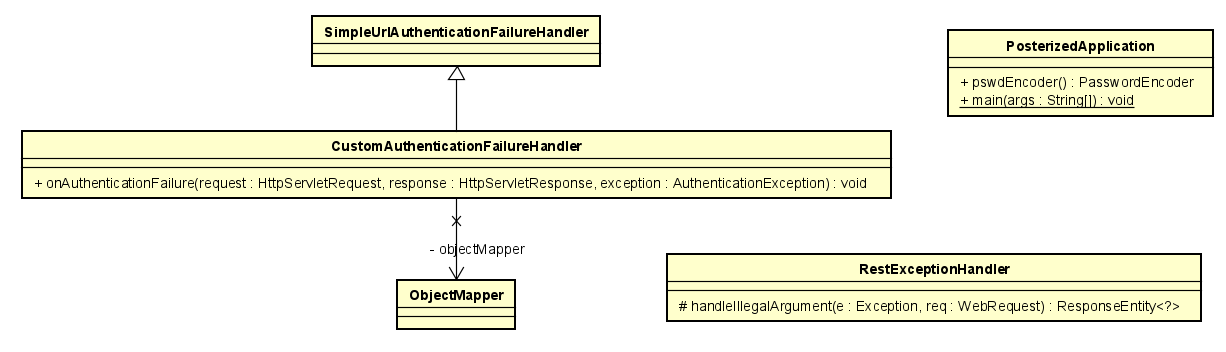
\includegraphics[scale=0.5]{dijagrami/glavni_4.png}%veličina slike u odnosu na originalnu datoteku i pozicija slike
				\centering
				\caption{Dijagram razreda - glavni dijagram 4.dio}
				\label{fig:promjena10.3}
			\end{figure}
			
			
			
			
			
			\eject
		
		\section{Dijagram stanja}
			
			
%			\textit{Potrebno je priložiti dijagram stanja i opisati ga. Dovoljan je jedan dijagram stanja koji prikazuje \textbf{značajan dio funkcionalnosti} sustava. Na primjer, stanja korisničkog sučelja i tijek korištenja neke ključne funkcionalnosti jesu značajan dio sustava, a registracija i prijava nisu. }

			Dijagram stanja je vrsta dijagrama koji se koristi u inženjerstvu softvera za prikazivanje različitih stanja kroz koja objekt ili interakcija prolazi tijekom svog životnog ciklusa. Obuhvaća stanja, prijelaze i događaje koji uzrokuju promjene iz jednog stanja u drugo. Korisan je u fazi dizajna jer pomaže u razumijevanju i vizualizaciji kako korisnici interagiraju s sustavom, te kako se sustav ponaša u različitim situacijama.
			
			\begin{figure}[H]
				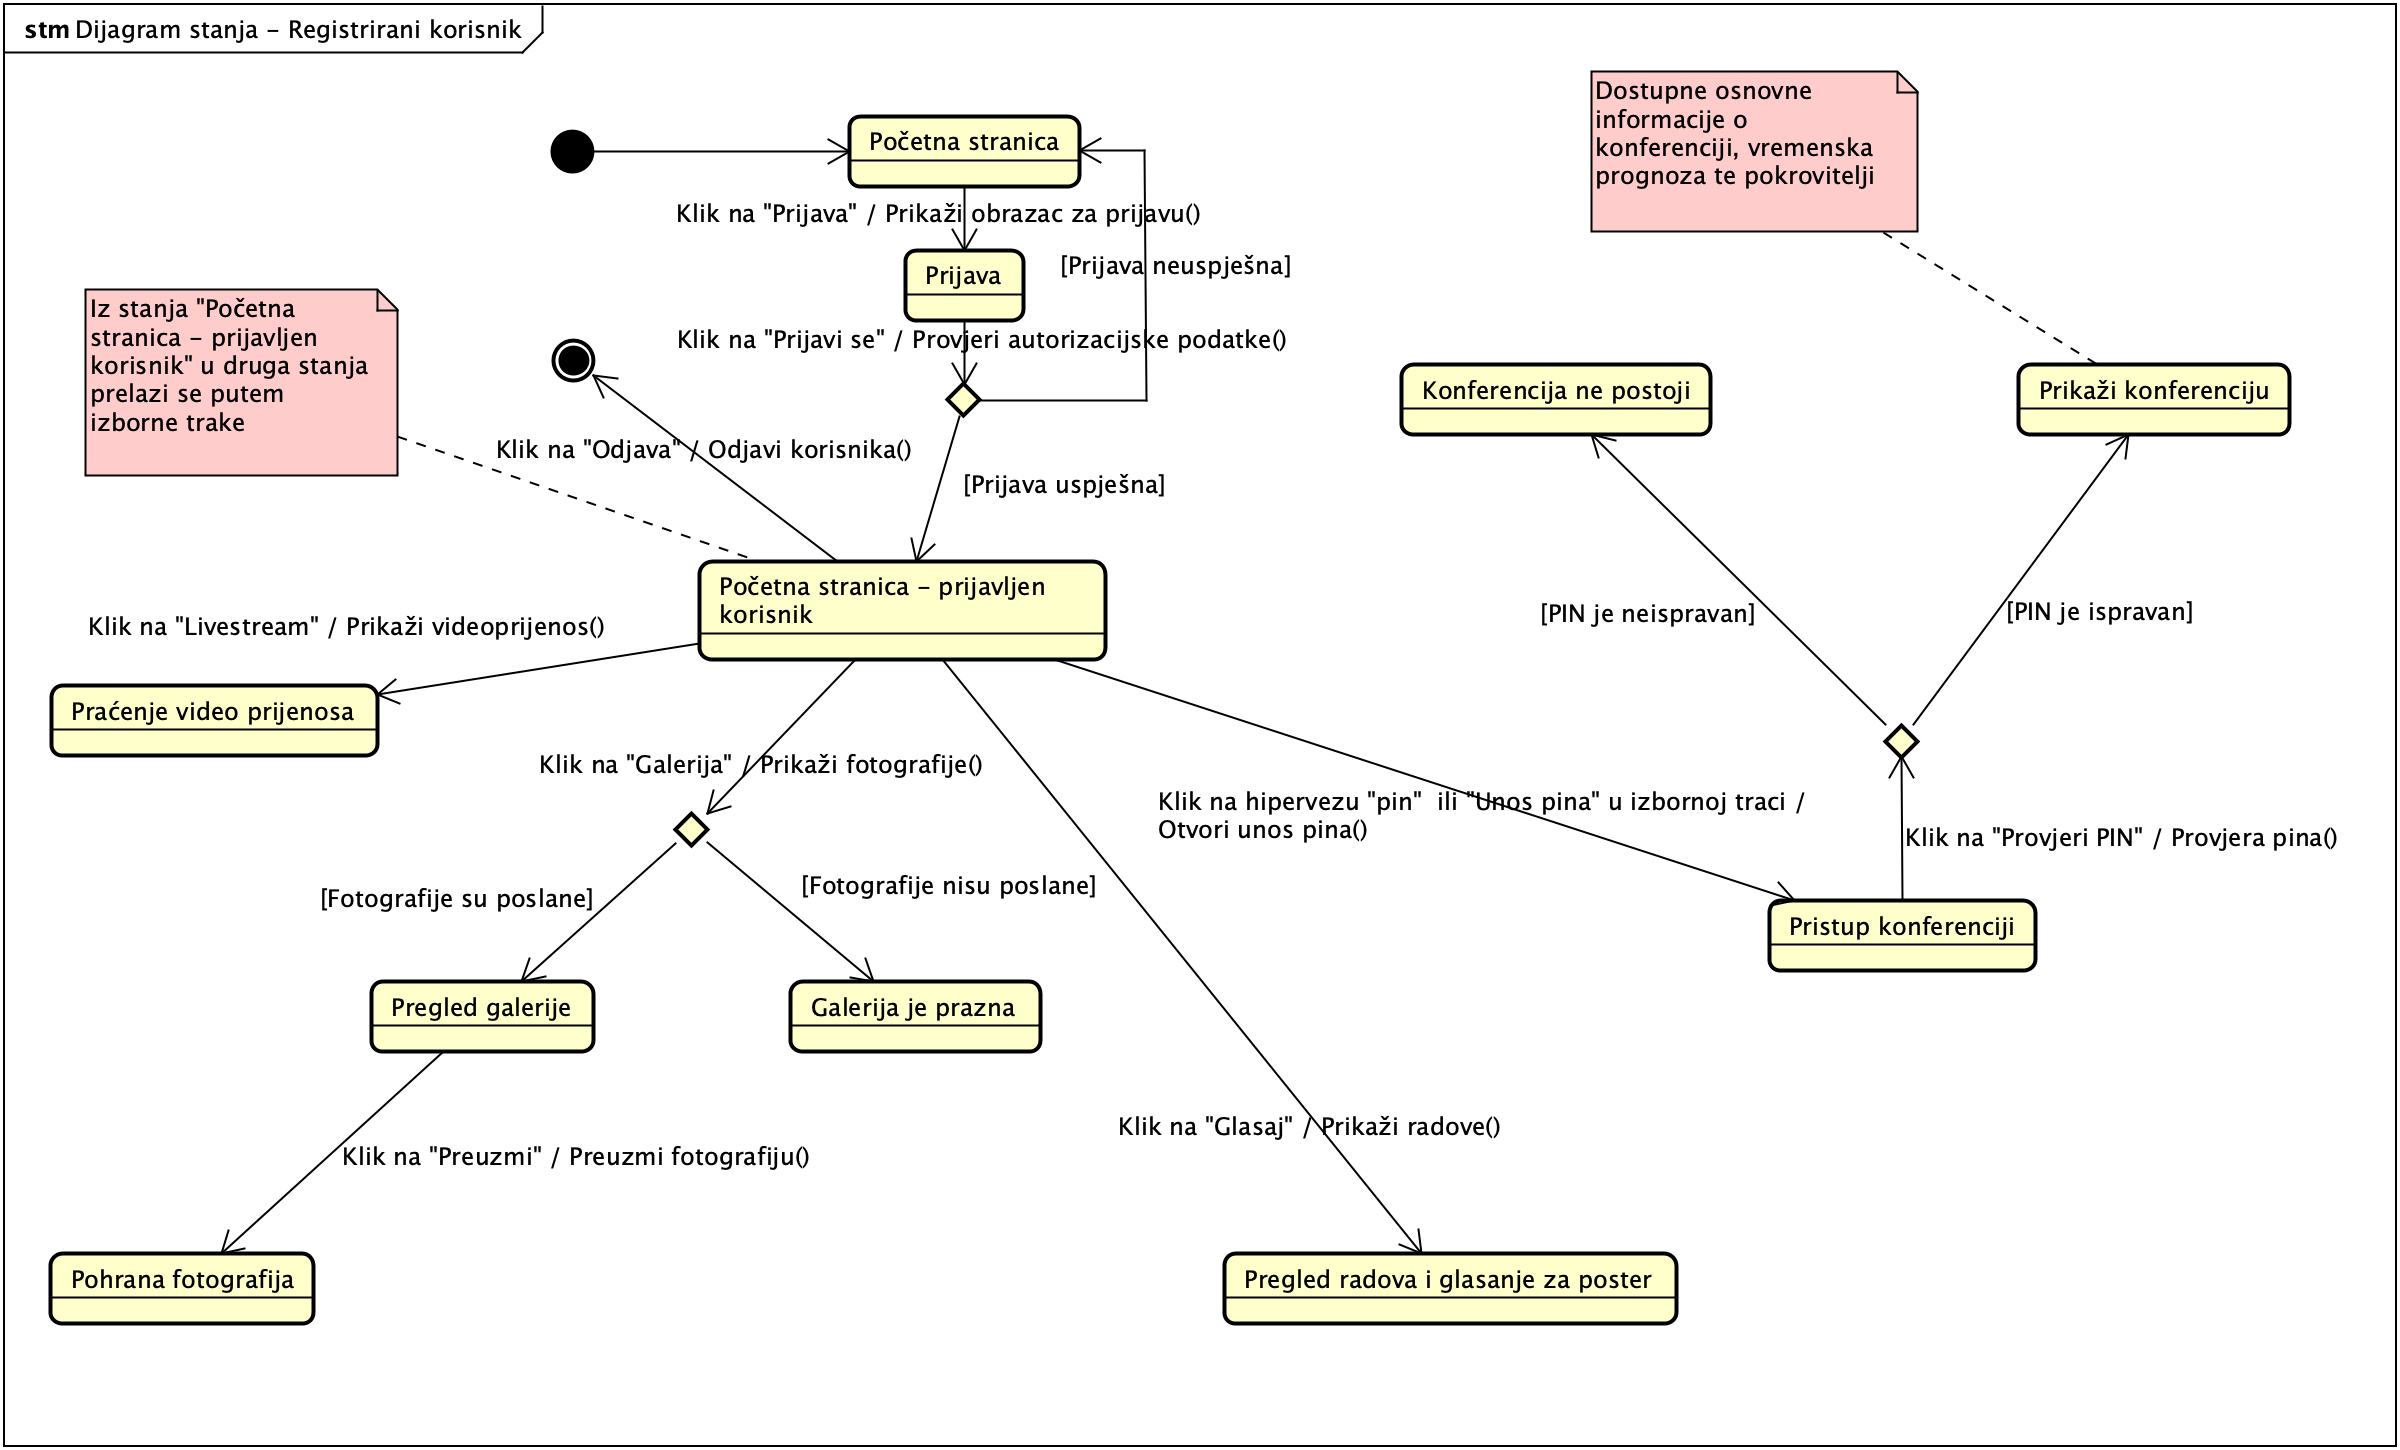
\includegraphics[scale=0.4]{dijagrami/dijagram_stanja.png} %veličina slike u odnosu na originalnu datoteku i pozicija slike
				\centering
				\caption{Dijagram stanja}
				\label{fig:promjene3}
			\end{figure}			
			
			
			\eject 
		
		\section{Dijagram aktivnosti}
			
			Dijagram aktivnosti primjenjuje se za opis modela toka upravljanja ili toka podataka. Ne upotrebljava se za modeliranje događajima poticanog ponašanja. U modeliranju toka upravljanja svaki novi korak poduzima se nakon završenog prethodnog, a naglasak je na jednostavnosti. Na dijagramu 4.8 prikazan je proces glasanja za najbolji rad. Registrirani korisnik se prijavljuje u sustav, a nakon uspješne prijave ima mogućnost prijaviti se na konferenciju. Korisnik se prijavljuje na konferenciju unosom pina te na web aplikaciji vidi mogućnosti povezane s tom konferencijom, uključujući i glasanje za najbolji rad. Odabire koji rad mu je najbolji te glasa za njega. 
			
			\begin{figure}[H]
				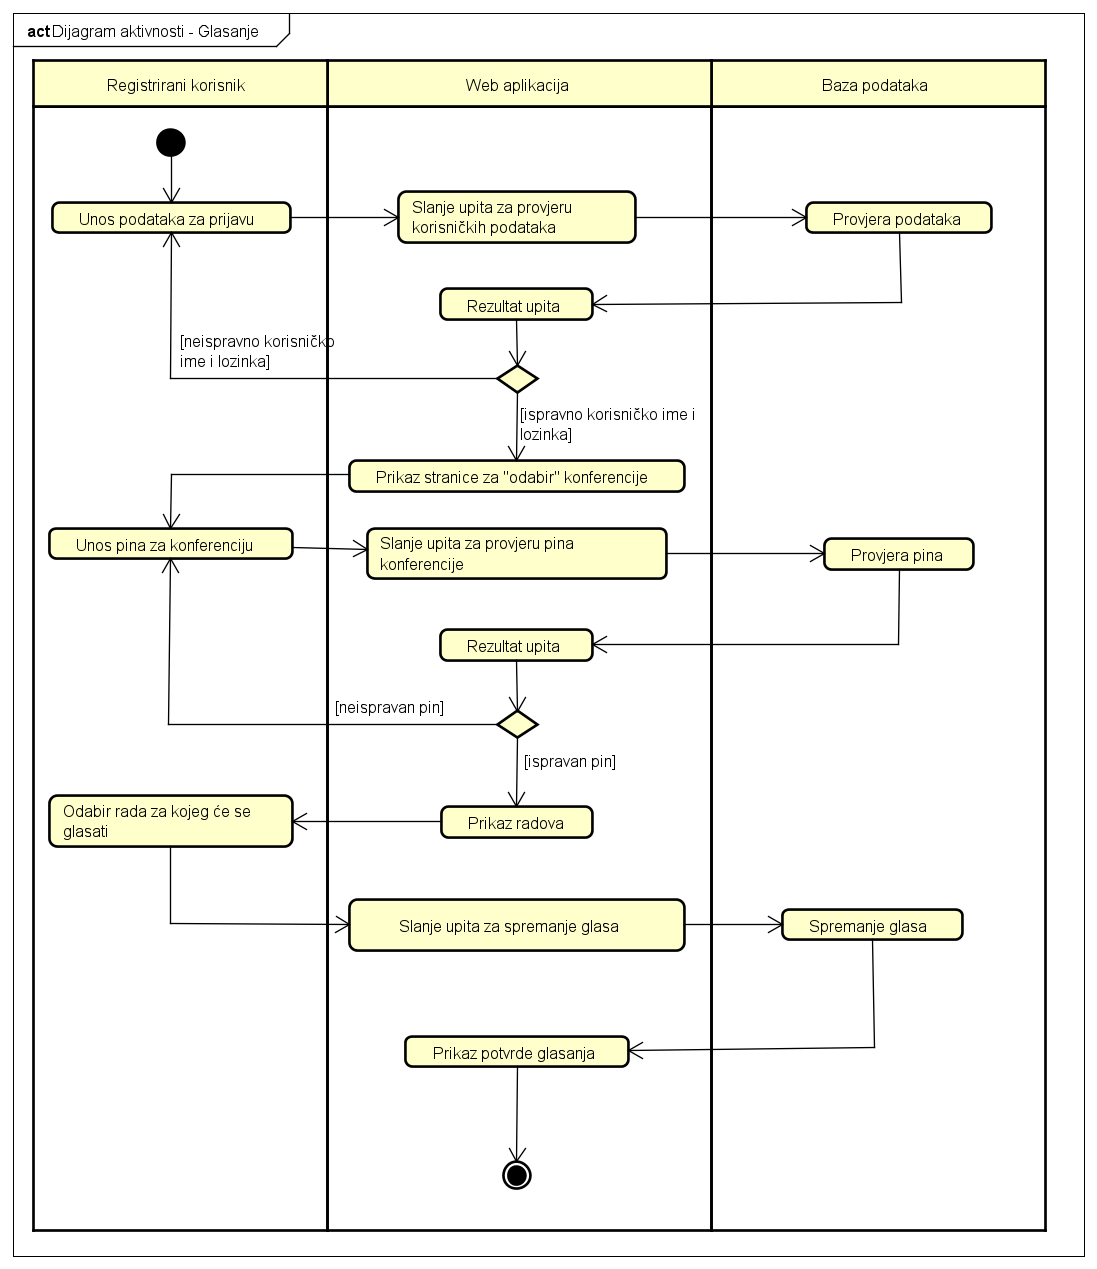
\includegraphics[scale=0.4]{dijagrami/dijagram_aktivnosti.png}%veličina slike u odnosu na originalnu datoteku i pozicija slike
			 	\centering
			 	\caption{Dijagram aktivnosti}
			 	\label{fig:promjene8.1}
			 \end{figure}
			 
			
			\eject
		\section{Dijagram komponenti}
		
			 Dijagram komponenti prikazan na slici opisuje strukturu web aplikacije razdijeljenu na višestruke komponente koje omogućavaju njen rad i interakciju s korisnicima. Pristup sustavu ostvaruje se putem dva osnovna sučelja.
			 
			 Prvo sučelje omogućava dohvat HTML, CSS i JS datoteka koje čine frontend dio aplikacije. Komponente frontenda koriste React biblioteku za izgradnju korisničkog sučelja i organizirane su u logičke cjeline prema tipovima korisnika koji im pristupaju, kao što su superadministratori, administratori, registrirani i neregistrirani korisnici.
			 
			 Router je ključna komponenta koja određuje koja će se datoteka poslužiti temeljem URL-a na koji korisnik dođe. Kroz ovu komponentu, zahtjevi korisnika se usmjeravaju prema odgovarajućim dijelovima aplikacije.
			 
			 Backend dio aplikacije pristupa se preko sučelja koje poslužuje JSON podatke. Ova komponenta se bavi obradom zahtjeva i komunikacijom s bazom podataka. Komunikacija s bazom podataka se odvija preko posebnog SQL API sučelja, a podaci se poslužuju kroz REST API.
			 
			 Svi dijelovi sustava su međusobno povezani i ovise o funkcionalnostima koje pružaju jedni drugima. Na primjer, REST API poslužuje kao most između frontenda i baze podataka, omogućavajući dinamičan i responzivan korisnički doživljaj. Dijagram detaljno prikazuje kako korisnički zahtjevi prolaze kroz različite slojeve aplikacije kako bi se dobili potrebni podaci ili izvršile akcije.
			 
			 \begin{figure}[H]
			 	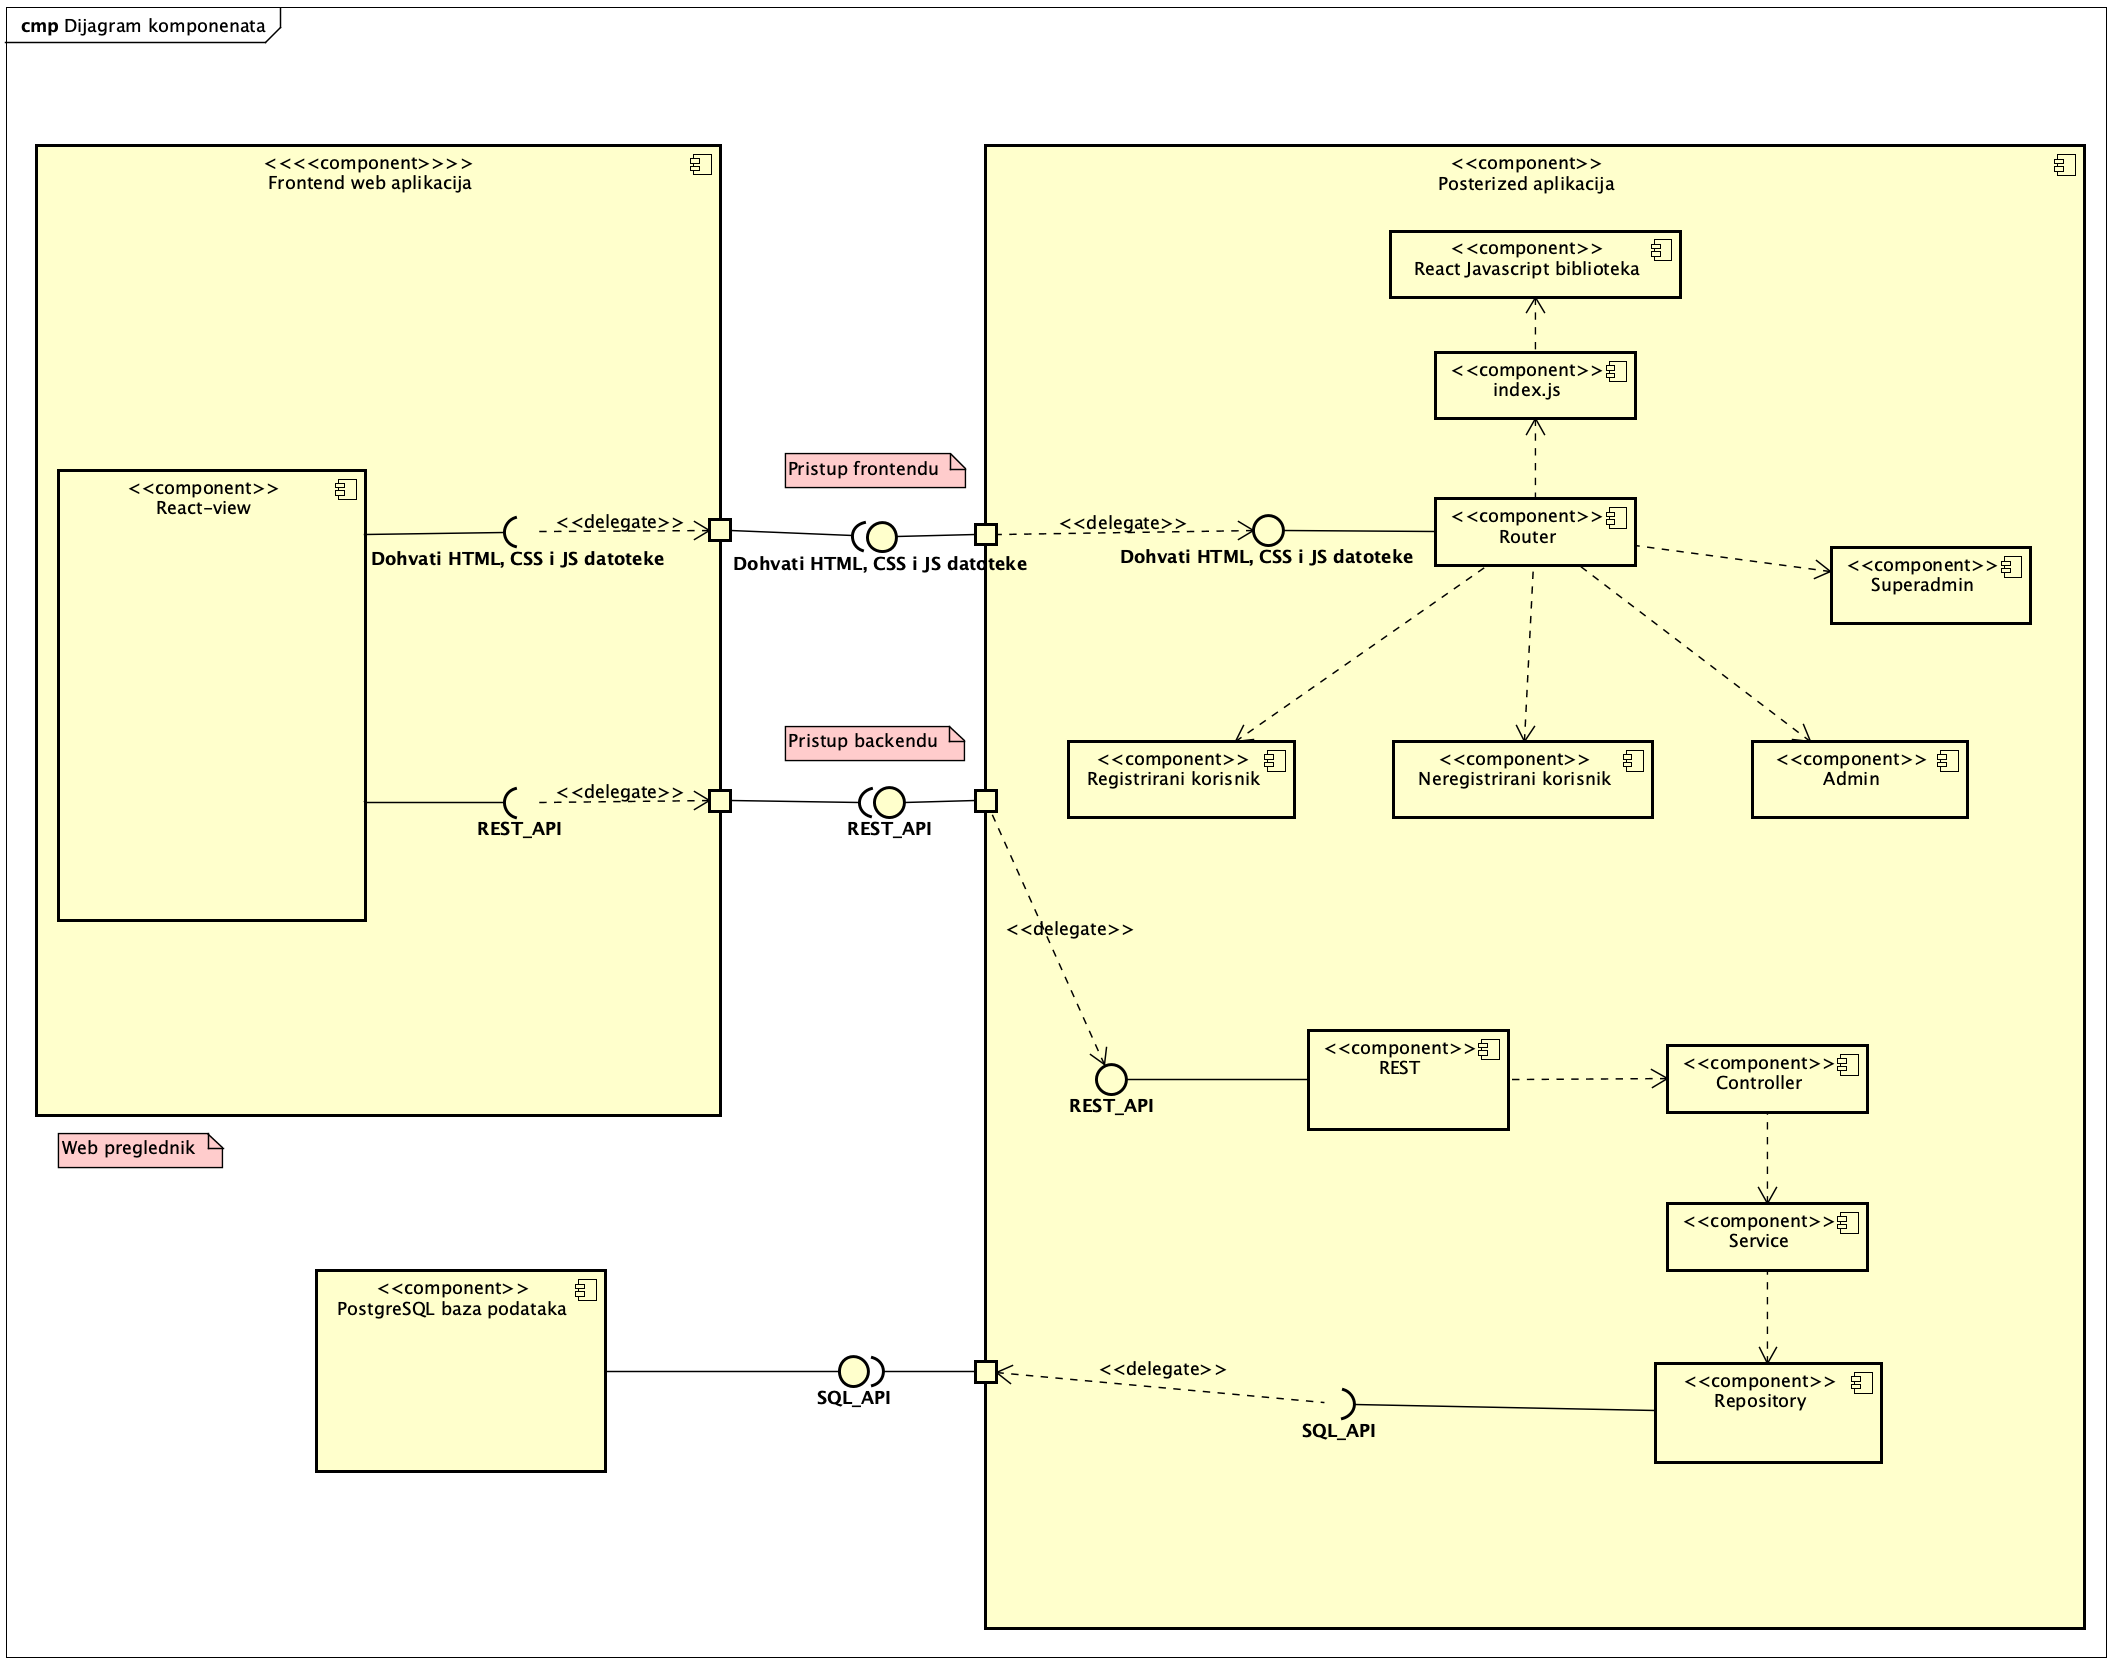
\includegraphics[scale=0.45]{dijagrami/dijagram_komponenata.png}%veličina slike u odnosu na originalnu datoteku i pozicija slike
			 	\centering
			 	\caption{Dijagram komponenata}
			 	\label{fig:promjene}
			 \end{figure}
		
	\chapter{Implementacija i korisničko sučelje}
		
		
		\section{Korištene tehnologije i alati}
		
			\textbf{\textit{dio 2. revizije}}
			
			 \textit{Detaljno navesti sve tehnologije i alate koji su primijenjeni pri izradi dokumentacije i aplikacije. Ukratko ih opisati, te navesti njihovo značenje i mjesto primjene. Za svaki navedeni alat i tehnologiju je potrebno \textbf{navesti internet poveznicu} gdje se mogu preuzeti ili više saznati o njima}.
			
			
			\eject 
		
	
		\section{Ispitivanje programskog rješenja}
			
			\textbf{\textit{dio 2. revizije}}\\
			
			 \textit{U ovom poglavlju je potrebno opisati provedbu ispitivanja implementiranih funkcionalnosti na razini komponenti i na razini cijelog sustava s prikazom odabranih ispitnih slučajeva. Studenti trebaju ispitati temeljnu funkcionalnost i rubne uvjete.}
	
			
			\subsection{Ispitivanje komponenti}
			\textit{Potrebno je provesti ispitivanje jedinica (engl. unit testing) nad razredima koji implementiraju temeljne funkcionalnosti. Razraditi \textbf{minimalno 6 ispitnih slučajeva} u kojima će se ispitati redovni slučajevi, rubni uvjeti te izazivanje pogreške (engl. exception throwing). Poželjno je stvoriti i ispitni slučaj koji koristi funkcionalnosti koje nisu implementirane. Potrebno je priložiti izvorni kôd svih ispitnih slučajeva te prikaz rezultata izvođenja ispita u razvojnom okruženju (prolaz/pad ispita). }
			
			
			
			\subsection{Ispitivanje sustava}
			
			 \textit{Potrebno je provesti i opisati ispitivanje sustava koristeći radni okvir Selenium\footnote{\url{https://www.seleniumhq.org/}}. Razraditi \textbf{minimalno 4 ispitna slučaja} u kojima će se ispitati redovni slučajevi, rubni uvjeti te poziv funkcionalnosti koja nije implementirana/izaziva pogrešku kako bi se vidjelo na koji način sustav reagira kada nešto nije u potpunosti ostvareno. Ispitni slučaj se treba sastojati od ulaza (npr. korisničko ime i lozinka), očekivanog izlaza ili rezultata, koraka ispitivanja i dobivenog izlaza ili rezultata.\\ }
			 
			 \textit{Izradu ispitnih slučajeva pomoću radnog okvira Selenium moguće je provesti pomoću jednog od sljedeća dva alata:}
			 \begin{itemize}
			 	\item \textit{dodatak za preglednik \textbf{Selenium IDE} - snimanje korisnikovih akcija radi automatskog ponavljanja ispita	}
			 	\item \textit{\textbf{Selenium WebDriver} - podrška za pisanje ispita u jezicima Java, C\#, PHP koristeći posebno programsko sučelje.}
			 \end{itemize}
		 	\textit{Detalji o korištenju alata Selenium bit će prikazani na posebnom predavanju tijekom semestra.}
			
			\eject 
		
		
		\section{Dijagram razmještaja}
			
			\textbf{\textit{dio 2. revizije}}
			
			 \textit{Potrebno je umetnuti \textbf{specifikacijski} dijagram razmještaja i opisati ga. Moguće je umjesto specifikacijskog dijagrama razmještaja umetnuti dijagram razmještaja instanci, pod uvjetom da taj dijagram bolje opisuje neki važniji dio sustava.}
			
			\eject 
		
		\section{Upute za puštanje u pogon}
		
			\textbf{\textit{dio 2. revizije}}\\
		
			 \textit{U ovom poglavlju potrebno je dati upute za puštanje u pogon (engl. deployment) ostvarene aplikacije. Na primjer, za web aplikacije, opisati postupak kojim se od izvornog kôda dolazi do potpuno postavljene baze podataka i poslužitelja koji odgovara na upite korisnika. Za mobilnu aplikaciju, postupak kojim se aplikacija izgradi, te postavi na neku od trgovina. Za stolnu (engl. desktop) aplikaciju, postupak kojim se aplikacija instalira na računalo. Ukoliko mobilne i stolne aplikacije komuniciraju s poslužiteljem i/ili bazom podataka, opisati i postupak njihovog postavljanja. Pri izradi uputa preporučuje se \textbf{naglasiti korake instalacije uporabom natuknica} te koristiti što je više moguće \textbf{slike ekrana} (engl. screenshots) kako bi upute bile jasne i jednostavne za slijediti.}
			
			
			 \textit{Dovršenu aplikaciju potrebno je pokrenuti na javno dostupnom poslužitelju. Studentima se preporuča korištenje neke od sljedećih besplatnih usluga: \href{https://aws.amazon.com/}{Amazon AWS}, \href{https://azure.microsoft.com/en-us/}{Microsoft Azure} ili \href{https://www.heroku.com/}{Heroku}. Mobilne aplikacije trebaju biti objavljene na F-Droid, Google Play ili Amazon App trgovini.}
			
			
			\eject 
	\chapter{Zaključak i budući rad}
		
		\textbf{\textit{dio 2. revizije}}\\
		
		 \textit{U ovom poglavlju potrebno je napisati osvrt na vrijeme izrade projektnog zadatka, koji su tehnički izazovi prepoznati, jesu li riješeni ili kako bi mogli biti riješeni, koja su znanja stečena pri izradi projekta, koja bi znanja bila posebno potrebna za brže i kvalitetnije ostvarenje projekta i koje bi bile perspektive za nastavak rada u projektnoj grupi.}
		
		 \textit{Potrebno je točno popisati funkcionalnosti koje nisu implementirane u ostvarenoj aplikaciji.}
		
		\eject 
	\chapter*{Popis literature}
		\addcontentsline{toc}{chapter}{Popis literature}
	 	
 		\textbf{\textit{Kontinuirano osvježavanje}}
	
		\textit{Popisati sve reference i literaturu koja je pomogla pri ostvarivanju projekta.}
		
		
		\begin{enumerate}
			
			
			\item  Programsko inženjerstvo, FER ZEMRIS, \url{http://www.fer.hr/predmet/proinz}
			
			\item  I. Sommerville, "Software engineering", 8th ed, Addison Wesley, 2007.
			
			\item  T.C.Lethbridge, R.Langaniere, "Object-Oriented Software Engineering", 2nd ed. McGraw-Hill, 2005.
			
			\item  I. Marsic, Software engineering book``, Department of Electrical and Computer Engineering, Rutgers University, \url{http://www.ece.rutgers.edu/~marsic/books/SE}
			
			\item  The Unified Modeling Language, \url{https://www.uml-diagrams.org/}
			
			\item  Astah Community, \url{http://astah.net/editions/uml-new}
		\end{enumerate}
		
		 
	
	
	\begingroup
	\renewcommand*\listfigurename{Indeks slika i dijagrama}
	%\renewcommand*\listtablename{Indeks tablica}
	%\let\clearpage\relax
	\listoffigures
	%\vspace{10mm}
	%\listoftables
	\endgroup
	\addcontentsline{toc}{chapter}{Indeks slika i dijagrama}


	
	\eject 
		
	\chapter*{Dodatak: Prikaz aktivnosti grupe}
		\addcontentsline{toc}{chapter}{Dodatak: Prikaz aktivnosti grupe}
		
		\section*{Dnevnik sastajanja}
		
		%\textbf{\textit{Kontinuirano osvježavanje}}\\
		
		 %\textit{U ovom dijelu potrebno je redovito osvježavati dnevnik sastajanja prema predlošku.}
		
		\begin{packed_enum}
			\item  sastanak
			
			\item[] \begin{packed_item}
				\item Datum: 19. listopada 2023.
				\item Prisustvovali: D.Barukčić, L.Barić, N.Božić, K.Đunđek, L.Jukić, E.Samaržija, T.Topolovec
				\item Teme sastanka:
				\begin{packed_item}
					\item  upoznavanje
					\item  diskusija na temu projekta 
				\end{packed_item}
			\end{packed_item}
			
			\item  sastanak
			\item[] \begin{packed_item}
				\item Datum: 20. listopada 2023.
				\item Prisustvovali: D.Barukčić, L.Barić, N.Božić, K.Đunđek, L.Jukić, E.Samaržija, T.Topolovec
				\item Teme sastanka:
				\begin{packed_item}
					\item  podjela poslova i grupiranje unutarnjih timova 
					\item  dogovaranje oko tehnologija koje će se koristiti u izradi projekta
				\end{packed_item}
			\end{packed_item}
			
			\item  sastanak
			\item[] \begin{packed_item}
				\item Datum: 26. listopada 2023.
				\item Prisustvovali: D.Barukčić, L.Barić, N.Božić, K.Đunđek, L.Jukić, E.Samaržija, T.Topolovec
				\item Teme sastanka:
				\begin{packed_item}
					\item  razrada backenda 
					\item  ideje o izgledu stranice
					
				\end{packed_item}
			\end{packed_item}
			
			\item  sastanak
			\item[] \begin{packed_item}
				\item Datum: 3. studenoga 2023.
				\item Prisustvovali: D.Barukčić, L.Barić, N.Božić, K.Đunđek, L.Jukić, E.Samaržija, T.Topolovec
				\item Teme sastanka:
				\begin{packed_item}
					\item  izrada stranice, homepagea, logina i registracije
					\item  testiranje backenda
				\end{packed_item}
			\end{packed_item}
			
			\item  sastanak
			\item[] \begin{packed_item}
				\item Datum: 15. studenoga 2023.
				\item Prisustvovali: D.Barukčić, L.Barić, N.Božić, K.Đunđek, L.Jukić, E.Samaržija, T.Topolovec
				\item Teme sastanka:
				\begin{packed_item}
					\item  rasprava o deployu
					\item  završavanje dokumentacije
					\item  problemi u backendu 
				\end{packed_item}
			\end{packed_item}
			
			%
			
		\end{packed_enum}
		
		\eject
		\section*{Tablica aktivnosti}
		
			%\textbf{\textit{Kontinuirano osvježavanje}}\\
			
			 %\textit{Napomena: Doprinose u aktivnostima treba navesti u satima po članovima grupe po aktivnosti.}

			\begin{longtblr}[
					label=none,
				]{
					vlines,hlines,
					width = \textwidth,
					colspec={X[7, l]X[1, c]X[1, c]X[1, c]X[1, c]X[1, c]X[1, c]X[1, c]}, 
					vline{1} = {1}{text=\clap{}},
					hline{1} = {1}{text=\clap{}},
					rowhead = 1,
				} 
				
				\SetCell[c=1]{c}{} & \SetCell[c=1]{c}{\rotatebox{90}{\textbf{Dominik Barukčić }}} & \SetCell[c=1]{c}{\rotatebox{90}{\textbf{Lana Barić }}} &	\SetCell[c=1]{c}{\rotatebox{90}{\textbf{Nika Božić }}} & \SetCell[c=1]{c}{\rotatebox{90}{\textbf{Kristina Đunđek }}} &	\SetCell[c=1]{c}{\rotatebox{90}{\textbf{Lovro Jukić }}} & \SetCell[c=1]{c}{\rotatebox{90}{\textbf{Ena Samaržija }}} &	\SetCell[c=1]{c}{\rotatebox{90}{\textbf{Tea Topolovec }}} \\  
				Upravljanje projektom               & 15 & 0 & 0 & 0 & 0 & 0 & 0 \\
				Opis projektnog zadatka            & 1  & 0 & 2 & 0 & 0 & 0 & 0 \\
				Funkcionalni zahtjevi              & 1  & 0 & 4 & 0 & 5 & 5 & 0 \\
				Opis pojedinih obrazaca            & 1  & 0 & 3 & 0 & 3 & 1 & 0 \\
				Dijagram obrazaca                  & 0  & 0 & 0 & 2 & 0 & 3 & 0 \\
				Sekvencijski dijagrami            & 0  & 2 & 0 & 3 & 0 & 0 & 0 \\
				Opis ostalih zahtjeva              & 0  & 3 & 0 & 0 & 0 & 0 & 0 \\
				Arhitektura i dizajn sustava       & 0  & 0 & 0 & 0 & 0 & 0 & 3 \\
				Baza podataka                      & 0  & 0 & 0 & 0 & 0 & 0 & 4 \\
				Dijagram razreda                   & 0  & 2 & 0 & 2 & 0 & 0 & 0 \\
				Dijagram stanja                    & 0  & 0 & 0 & 0 & 0 & 0 & 0 \\
				Dijagram aktivnosti                & 0  & 0 & 0 & 0 & 0 & 0 & 0 \\
				Dijagram komponenti                & 2  & 0 & 0 & 0 & 0 & 0 & 0 \\
				Korištene tehnologije i alati      & 1  & 0 & 0 & 0 & 0 & 0 & 0 \\
				Ispitivanje programskog rješenja   & 0  & 0 & 0 & 0 & 0 & 0 & 0 \\
				Dijagram razmještaja               & 1  & 0 & 0 & 0 & 0 & 0 & 0 \\
				Upute za puštanje u pogon          & 2  & 0 & 0 & 0 & 0 & 0 & 0 \\
				Dnevnik sastajanja                & 1  & 0 & 0 & 0 & 0 & 0 & 0 \\
				Zaključak i budući rad            & 2  & 0 & 0 & 0 & 0 & 0 & 0 \\
				Popis literature                  & 1  & 0 & 0 & 0 & 0 & 0 & 0 \\
				\textit{izrada baze podataka} 		 			& 0 & 0 & 0 & 0 & 0 & 0 & 4 \\  
				\textit{back end} 							& 0 & 13 & 0 & 14 & 0 & 0 & 11 \\  
				\textit{front end} 							& 0 & 13 & 0 & 14 & 0 & 0 & 11 \\  
				\textit{deploy} 							& 20 & 0 & 0 & 0 & 0 & 0 & 0 \\ 
			\end{longtblr}
					
					
		\eject
		\section*{Dijagrami pregleda promjena}
		
		\textbf{\textit{dio 2. revizije}}\\
		
		\textit{Prenijeti dijagram pregleda promjena nad datotekama projekta. Potrebno je na kraju projekta generirane grafove s gitlaba prenijeti u ovo poglavlje dokumentacije. Dijagrami za vlastiti projekt se mogu preuzeti s gitlab.com stranice, u izborniku Repository, pritiskom na stavku Contributors.}
		
	


\end{document} %naredbe i tekst nakon ove naredbe ne ulaze u izgrađen dokument 


